% !TeX spellcheck = hu_HU
% !TeX encoding = UTF-8
% !TeX program = xelatex
\documentclass[11pt,a4paper,oneside]{report}             % Single-side
%\documentclass[11pt,a4paper,twoside,openright]{report}  % Duplex

\usepackage{tikz}
\usetikzlibrary{positioning,arrows.meta,shapes.geometric,fit,calc,backgrounds,babel}
\usepackage{pgfplots}
\pgfplotsset{compat=1.17}
\usepgfplotslibrary{colormaps}

% thanks to http://tex.stackexchange.com/a/47579/71109
\usepackage{ifxetex}
\usepackage{ifluatex}
\newif\ifxetexorluatex % a new conditional starts as false
\ifnum 0\ifxetex 1\fi\ifluatex 1\fi>0
   \xetexorluatextrue
\fi

\ifxetexorluatex
  \usepackage{fontspec}
\else
  \usepackage[T1]{fontenc}
  \usepackage[utf8]{inputenc}
  \usepackage[lighttt]{lmodern}
\fi

\usepackage[english,magyar]{babel} % Alapértelmezés szerint utoljára definiált nyelv lesz aktív, de később külön beállítjuk az aktív nyelvet.

%\usepackage{cmap}
\usepackage{amsfonts,amsmath,amssymb} % Mathematical symbols.
%\usepackage[ruled,boxed,resetcount,linesnumbered]{algorithm2e} % For pseudocodes. % beware: this is not compatible with LuaLaTeX, see http://tex.stackexchange.com/questions/34814/lualatex-and-algorithm2e
\usepackage{booktabs} % For publication quality tables for LaTeX
\usepackage{graphicx}

%\usepackage{fancyhdr}
%\usepackage{lastpage}

\usepackage{anysize}
%\usepackage{sectsty}
\usepackage{setspace} % For setting line spacing

\usepackage[unicode]{hyperref} % For hyperlinks in the generated document.
\usepackage{xcolor}
\usepackage{listings} % For source code snippets.

\usepackage[amsmath,thmmarks]{ntheorem} % Theorem-like environments.

\usepackage[hang]{caption}

\singlespacing

\newcommand{\selecthungarian}{
	\selectlanguage{magyar}
	\setlength{\parindent}{2em}
	\setlength{\parskip}{0em}
	\frenchspacing
}

\newcommand{\selectenglish}{
	\selectlanguage{english}
	\setlength{\parindent}{0em}
	\setlength{\parskip}{0.5em}
	\nonfrenchspacing
	\renewcommand{\figureautorefname}{Figure}
	\renewcommand{\tableautorefname}{Table}
	\renewcommand{\partautorefname}{Part}
	\renewcommand{\chapterautorefname}{Chapter}
	\renewcommand{\sectionautorefname}{Section}
	\renewcommand{\subsectionautorefname}{Section}
	\renewcommand{\subsubsectionautorefname}{Section}
}

\usepackage[numbers]{natbib}
\usepackage{xspace}


\usepackage{multirow}
\usepackage{tabularx}
\usepackage{float}

\newcommand{\screenshot}[3]{%
	\IfFileExists{figures/#1}%
		{\includegraphics[#3]{figures/#1}}%
		{\fbox{\parbox[c][4.5cm][c]{0.44\linewidth}{\centering\small Képernyőkép helye:\\ \texttt{figures/\detokenize{#1}}\\[2mm] \footnotesize #2}}}%
}

\newcommand{\vikszerzoVezeteknev}{Székely}
\newcommand{\vikszerzoKeresztnev}{Máté Zsombor}

\newcommand{\vikkonzulensAMegszolitas}{}
\newcommand{\vikkonzulensAVezeteknev}{Szekeres}
\newcommand{\vikkonzulensAKeresztnev}{Kornél}

\newcommand{\vikkonzulensBMegszolitas}{}
\newcommand{\vikkonzulensBVezeteknev}{}
\newcommand{\vikkonzulensBKeresztnev}{}

\newcommand{\vikkonzulensCMegszolitas}{}
\newcommand{\vikkonzulensCVezeteknev}{}
\newcommand{\vikkonzulensCKeresztnev}{}

\newcommand{\vikcim}{Sakkrobot fejlesztése és adaptálása új bábuk kezelésére} % Cím
\newcommand{\viktanszek}{\bmeaut} % Tanszék
\newcommand{\vikdoktipus}{\bsc} % Dokumentum típusa (\bsc vagy \msc)
\newcommand{\vikmunkatipusat}{szakdolgozatot} % a "hallgató nyilatkozat" részhez: szakdolgozatot vagy diplomatervet

%--------------------------------------------------------------------------------------
% TDK-specifikus változók
%--------------------------------------------------------------------------------------
\newcommand{\tdkszerzoB}{Második Szerző} % Második szerző neve; hagyd üresen, ha egyedül írtad a TDK-t.
\newcommand{\tdkev}{2014} % A dolgozat írásának éve (pl. "2014") (Ez OTDK-nál eltérhet az aktuális évtől.)

% További adatok az OTDK címlaphoz (BME-s TDK-hoz nem kell kitölteni)
\newcommand{\tdkevfolyamA}{IV} % Első szerző évfolyama, római számmal (pl. IV).
\newcommand{\tdkevfolyamB}{III} % Második szerző évfolyama, római számmal (pl. III).
\newcommand{\tdkkonzulensbeosztasA}{egyetemi tanár} % Első konzulens beosztása (pl. egyetemi docens)
\newcommand{\tdkkonzulensbeosztasB}{doktorandusz} % Második konzulens beosztása (pl. egyetemi docens)

\newcommand{\szerzoMeta}{\vikszerzoVezeteknev{} \vikszerzoKeresztnev} % egy szerző esetén

% Beállítások magyar nyelvű dolgozathoz
%--------------------------------------------------------------------------------------
% Elnevezések
%--------------------------------------------------------------------------------------
\newcommand{\bme}{Budapesti Műszaki és Gazdaságtudományi Egyetem}
\newcommand{\vik}{Villamosmérnöki és Informatikai Kar}

\newcommand{\bmemit}{Méréstechnika és Információs Rendszerek Tanszék}

\newcommand{\keszitette}{Készítette}
\newcommand{\konzulens}{Konzulens}

\newcommand{\bsc}{Szakdolgozat}
\newcommand{\msc}{Diplomaterv}
\newcommand{\tdk}{TDK dolgozat}
\newcommand{\bsconlab}{BSc Önálló laboratórium}
\newcommand{\msconlabi}{MSc Önálló laboratórium 1.}
\newcommand{\msconlabii}{MSc Önálló laboratórium 2.}

\newcommand{\pelda}{Példa}
\newcommand{\definicio}{Definíció}
\newcommand{\tetel}{Tétel}

\newcommand{\bevezetes}{Bevezetés}
\newcommand{\koszonetnyilvanitas}{Köszönetnyilvánítás}
\newcommand{\fuggelek}{Függelék}

% Opcionálisan átnevezhető címek
%\addto\captionsmagyar{%
%\renewcommand{\listfigurename}{Saját ábrajegyzék cím}
%\renewcommand{\listtablename}{Saját táblázatjegyzék cím}
%\renewcommand{\bibname}{Saját irodalomjegyzék név}
%}

\newcommand{\szerzo}{\vikszerzoVezeteknev{} \vikszerzoKeresztnev}
\newcommand{\vikkonzulensA}{\vikkonzulensAMegszolitas\vikkonzulensAVezeteknev{} \vikkonzulensAKeresztnev}
\newcommand{\vikkonzulensB}{\vikkonzulensBMegszolitas\vikkonzulensBVezeteknev{} \vikkonzulensBKeresztnev}
\newcommand{\vikkonzulensC}{\vikkonzulensCMegszolitas\vikkonzulensCVezeteknev{} \vikkonzulensCKeresztnev}

\newcommand{\selectthesislanguage}{\selecthungarian}

\bibliographystyle{huplain}

\def\lstlistingname{lista}

\newcommand{\appendixnumber}{6}  % a fofejezet-szamlalo az angol ABC 6. betuje (F) lesz

\newcommand{\declaration}{declaration_HU}
\newcommand{\AIdeclaration}{AI_nyilatkozat_tablazat_HU}

\newcommand{\bmeaut}{Automatizálási és Alkalmazott Informatikai Tanszék}

%--------------------------------------------------------------------------------------
% Page layout setup
%--------------------------------------------------------------------------------------
% we need to redefine the pagestyle plain
% another possibility is to use the body of this command without \fancypagestyle
% and use \pagestyle{fancy} but in that case the special pages
% (like the ToC, the References, and the Chapter pages)remain in plane style

\pagestyle{plain}
\marginsize{35mm}{25mm}{15mm}{15mm}

\setcounter{tocdepth}{3}
%\sectionfont{\large\upshape\bfseries}
\setcounter{secnumdepth}{3}

\sloppy % Margón túllógó sorok tiltása.
\widowpenalty=10000 \clubpenalty=10000 %A fattyú- és árvasorok elkerülése
\def\hyph{-\penalty0\hskip0pt\relax} % Kötőjeles szavak elválasztásának engedélyezése


%--------------------------------------------------------------------------------------
% Setup hyperref package
%--------------------------------------------------------------------------------------
\hypersetup{
    % bookmarks=true,            % show bookmarks bar?
    unicode=true,              % non-Latin characters in Acrobat's bookmarks
    pdftitle={\vikcim},        % title
    pdfauthor={\szerzoMeta},    % author
    pdfsubject={\vikdoktipus}, % subject of the document
    pdfcreator={\szerzoMeta},   % creator of the document
    pdfproducer={},    % producer of the document
    pdfkeywords={},    % list of keywords (separate then by comma)
    pdfnewwindow=true,         % links in new window
    colorlinks=true,           % false: boxed links; true: colored links
    linkcolor=black,           % color of internal links
    citecolor=black,           % color of links to bibliography
    filecolor=black,           % color of file links
    urlcolor=black             % color of external links
}


%--------------------------------------------------------------------------------------
% Set up listings
%--------------------------------------------------------------------------------------
\definecolor{lightgray}{rgb}{0.95,0.95,0.95}
\lstset{
	basicstyle=\scriptsize\ttfamily, % print whole listing small
	keywordstyle=\color{black}\bfseries, % bold black keywords
	identifierstyle=, % nothing happens
	% default behavior: comments in italic, to change use
	% commentstyle=\color{green}, % for e.g. green comments
	stringstyle=\scriptsize,
	showstringspaces=false, % no special string spaces
	aboveskip=3pt,
	belowskip=3pt,
	backgroundcolor=\color{lightgray},
	columns=flexible,
	keepspaces=true,
	escapeinside={(*@}{@*)},
	captionpos=b,
	breaklines=true,
	frame=single,
	float=!ht,
	tabsize=2,
	literate=*
		{á}{{\'a}}1	{é}{{\'e}}1	{í}{{\'i}}1	{ó}{{\'o}}1	{ö}{{\"o}}1	{ő}{{\H{o}}}1	{ú}{{\'u}}1	{ü}{{\"u}}1	{ű}{{\H{u}}}1
		{Á}{{\'A}}1	{É}{{\'E}}1	{Í}{{\'I}}1	{Ó}{{\'O}}1	{Ö}{{\"O}}1	{Ő}{{\H{O}}}1	{Ú}{{\'U}}1	{Ü}{{\"U}}1	{Ű}{{\H{U}}}1
}


%--------------------------------------------------------------------------------------
% Set up theorem-like environments
%--------------------------------------------------------------------------------------
% Using ntheorem package -- see http://www.math.washington.edu/tex-archive/macros/latex/contrib/ntheorem/ntheorem.pdf

\theoremstyle{plain}
\theoremseparator{.}
\newtheorem{example}{\pelda}

\theoremseparator{.}
%\theoremprework{\bigskip\hrule\medskip}
%\theorempostwork{\hrule\bigskip}
\theorembodyfont{\upshape}
\theoremsymbol{{\large \ensuremath{\centerdot}}}
\newtheorem{definition}{\definicio}

\theoremseparator{.}
%\theoremprework{\bigskip\hrule\medskip}
%\theorempostwork{\hrule\bigskip}
\newtheorem{theorem}{\tetel}


%--------------------------------------------------------------------------------------
% Some new commands and declarations
%--------------------------------------------------------------------------------------
\newcommand{\code}[1]{{\upshape\ttfamily\scriptsize\indent #1}}
\newcommand{\doi}[1]{DOI: \href{http://dx.doi.org/\detokenize{#1}}{\raggedright{\texttt{\detokenize{#1}}}}} % A hivatkozások közt így könnyebb DOI-t megadni.

\DeclareMathOperator*{\argmax}{arg\,max}
%\DeclareMathOperator*[1]{\floor}{arg\,max}
\DeclareMathOperator{\sign}{sgn}
\DeclareMathOperator{\rot}{rot}


%--------------------------------------------------------------------------------------
% Setup captions
%--------------------------------------------------------------------------------------
\captionsetup[figure]{
	width=.75\textwidth,
	aboveskip=10pt}

\renewcommand{\captionlabelfont}{\bf}
%\renewcommand{\captionfont}{\footnotesize\it}

%--------------------------------------------------------------------------------------
% Hyphenation exceptions
%--------------------------------------------------------------------------------------
\hyphenation{Shakes-peare Mar-seilles ár-víz-tű-rő tü-kör-fú-ró-gép}


\author{\vikszerzo}
\title{\viktitle}

%--------------------------------------------------------------------------------------
% Table of contents and the main text
%--------------------------------------------------------------------------------------
\begin{document}

\pagenumbering{gobble}

\selectthesislanguage

\hypersetup{pageanchor=false}
%--------------------------------------------------------------------------------------
%	The title page
%--------------------------------------------------------------------------------------
\begin{titlepage}
\begin{center}

\includegraphics[width=60mm,keepaspectratio]{figures/bme_logo.pdf}\\
\vspace{0.3cm}
\textbf{\bme}\\
\textmd{\vik}\\
\textmd{\viktanszek}\\[5cm]

\vspace{0.4cm}
{\huge \bfseries \vikcim}\\[0.8cm]
\vspace{0.5cm}
\textsc{\Large \vikdoktipus}\\[4cm]

{
	\renewcommand{\arraystretch}{0.85}
	\begin{tabular}{cc}
	 \makebox[7cm]{\emph{\keszitette}} & \makebox[7cm]{\emph{\konzulens}} \\ \noalign{\smallskip}
	 \makebox[7cm]{\szerzo} & \makebox[7cm]{\vikkonzulensA} \\
	  & \makebox[7cm]{\vikkonzulensB} \\
	  & \makebox[7cm]{\vikkonzulensC} \\
	\end{tabular}
}

\vfill
{\large \today}
\end{center}
\end{titlepage}
\hypersetup{pageanchor=false}

		   % Szakdolgozat/Diplomaterv címlap

% Table of Contents
%~~~~~~~~~~~~~~~~~~~~~~~~~~~~~~~~~~~~~~~~~~~~~~~~~~~~~~~~~~~~~~~~~~~~~~~~~~~~~~~~~~~~~~
\tableofcontents\vfill

% Declaration and Abstract
%~~~~~~~~~~~~~~~~~~~~~~~~~~~~~~~~~~~~~~~~~~~~~~~~~~~~~~~~~~~~~~~~~~~~~~~~~~~~~~~~~~~~~~
\include{include/\declaration}
\pagenumbering{roman}
\setcounter{page}{1}

\selecthungarian

%----------------------------------------------------------------------------
% Abstract in Hungarian
%----------------------------------------------------------------------------
\chapter*{Kivonat}\addcontentsline{toc}{chapter}{Kivonat}

A szakdolgozatban egy saját fejlesztésű, C++20 nyelvű sakkmotort mutatok be, amely a klasszikus FIDE-szabályok mellett tündérsakk-bábuk kezelésére is képes. A motor bitboard-alapú táblareprezentációt és mágikus bitboardokkal gyorsított lépésgenerátort használ, döntéseit alfa-béta alapú kereséssel hozza, amelyet transzpozíciós tábla, PVS, aspirációs ablak, többféle vágási, redukciós és kiterjesztési technika, többszálú (Lazy SMP) keresés, valamint NNUE neurális hálós állásértékelés egészít ki. A sakkprogram HalfKP (régebbi verzió) mellett HalfKAv2 hálót is támogat. A motor szabványos UCI protokollon kommunikál, és saját, Qt~6 alapú grafikus felülettel rendelkezik, amely négy nehézségi szintet, sakkórát, lépésvisszavonást és játszma-visszajátszást is kínál.

A kereső fejlődését verziókezelt, robot-robot mérésekkel követtem: húsz mérés, összesen több mint tizenkétezer játszma igazolja az egyes optimalizációk hatását. A lépésgenerálás helyességét öt szabványos perft-tesztállás igazolja, egy szálon másodpercenként 25--33 millió állással. A korlátozott erősségű Stockfish~17.1 elleni 300 játszma alapján a motor ereje a CCRL blitz skálán kb. 3100 Elo. A tündérsakk-kiterjesztést az Amazon (vezér + huszár) bábun keresztül valósítottam meg: a bábu a lépésgenerátortól az értékelésen át a felületig minden réteget érint, mégis kevés, jól körülhatárolt módosítással illeszkedett a meglévő architektúrába. A dolgozat végül önjátszmák alapján elemzi, hogyan használja a kereső az új bábut.

\vfill
\selectenglish

%----------------------------------------------------------------------------
% Abstract in English
%----------------------------------------------------------------------------
\chapter*{Abstract}\addcontentsline{toc}{chapter}{Abstract}

This thesis presents a chess engine written from scratch in C++20 that plays by the classical FIDE rules and can also handle fairy chess pieces. The engine uses a bitboard board representation with a magic-bitboard move generator. Its decisions come from an alpha-beta search extended with a transposition table, principal variation search, aspiration windows, a range of pruning, reduction and extension techniques, multi-threaded (Lazy SMP) search and NNUE neural network evaluation, supporting both HalfKP (older version) and HalfKAv2 network. The engine communicates through the standard UCI protocol and has its own Qt~6 graphical user interface with four difficulty levels, chess clocks, move takeback and game review.

The development of the search was tracked with versioned bot-versus-bot measurements: twenty matches with more than twelve thousand games quantify the effect of each optimization. The correctness of the move generator is verified on five standard perft positions, running at 25--33 million positions per second on a single thread. Based on 300 games against strength-limited Stockfish~17.1, the engine plays at about 3100 Elo on the CCRL blitz scale. The fairy chess extension was implemented through the Amazon (queen + knight) piece. Although the piece affects every layer from move generation through evaluation to the user interface, it fit into the existing architecture with a small number of well-contained changes. Finally, the thesis analyses self-play games to show how the search makes use of the new piece.

\vfill
\selectthesislanguage

\newcounter{romanPage}
\setcounter{romanPage}{\value{page}}
\stepcounter{romanPage}


% The main part of the thesis
%~~~~~~~~~~~~~~~~~~~~~~~~~~~~~~~~~~~~~~~~~~~~~~~~~~~~~~~~~~~~~~~~~~~~~~~~~~~~~~~~~~~~~~
\pagenumbering{arabic}

%----------------------------------------------------------------------------
\chapter{\bevezetes}
%----------------------------------------------------------------------------

A sakk évtizedek óta a mesterséges intelligencia kutatásának egyik kedvelt terepe: szabályai pontosan definiáltak, állapottere azonban olyan hatalmas, hogy a teljes játékfa bejárása gyakorlatilag lehetetlen. Claude Shannon már 1950-ben megfogalmazta a számítógépes sakk alapproblémáját, és megbecsülte, hogy egy átlagos játszma lehetséges folytatásainak száma nagyságrendileg $10^{120}$~\cite{Shannon50}. Egy erős sakkmotor ezért nem brute-force kereséssel, hanem jól megválasztott vágási és értékelési heurisztikákkal dolgozik.

A szakdolgozatom célja egy saját fejlesztésű sakkmotor megtervezése és megvalósítása volt, amely
\begin{itemize}
	\item a klasszikus (FIDE) szabályok szerint játszik,
	\item az iparági szabványnak tekinthető UCI (Universal Chess Interface) protokollon keresztül más programokkal is együttműködik,
	\item saját, interaktív grafikus felhasználói felülettel rendelkezik,
	\item és úgy épül fel, hogy új, nem szabványos (tündérsakk) bábukkal is bővíthető legyen.
\end{itemize}

A tündérsakk-kiterjesztés bemutatására az Amazon bábut választottam, amely a vezér és a huszár lépésmódját egyesíti. Egy ilyen bábu bevezetése nemcsak a lépésgenerátort érinti, hanem a cserék kiértékelését, a lépésrendezést és az állásértékelést is, így jól megmutatja, mennyire általános egy motor architektúrája.

A munka két forráskód-tárolóban készült. A backend a motor konzolos változata, ebben fut a UCI és a robot-robot elleni tömeges mérés. A GUI projekt ugyanezt a motort egy grafikus felülettel egészíti ki. A fejlesztés 2025 decemberében indult, a motor 2026 áprilisától kezdve mért, verziózott lépésekben fejlődött: minden módosított keresőt egy korábbi verzió ellen több ezer játszmában teszteltem, és csak a bizonyítottan erősebb változatot tartottam meg.

\section*{A dolgozat felépítése}

\Aref{chap:rules}. fejezet bemutatja a vonatkozó FIDE-szabályokat és a tündérsakk bábuk alapelveit. \Aref{chap:background}. fejezet a sakkmotorok szakirodalmi hátterét foglalja össze. \Aref{chap:architecture}. fejezet a szoftverarchitektúrát és a UCI kommunikációs réteget, \aref{chap:movegen}. fejezet a táblareprezentációt és a lépésgenerálást ismerteti. \Aref{chap:search}. fejezet a keresőmotor összes funkcióját és optimalizációját tárgyalja, verziók szerint. \Aref{chap:gui}. fejezet a grafikus felületet, \aref{chap:amazon}. fejezet az Amazon bábuval bővített játékváltozatot mutatja be. \Aref{chap:measurements}. fejezetben mérésekkel igazolom a lépésgenerálás helyességét és hatékonyságát, valamint a motor fejlődését. A dolgozatot az eredmények értékelése és a továbbfejlesztési lehetőségek zárják.

%----------------------------------------------------------------------------
\chapter{Sakkszabályok és tündérsakk}\label{chap:rules}
%----------------------------------------------------------------------------

\section{A FIDE-szabályok motor szempontjából fontos részei}

A motor a Nemzetközi Sakkszövetség (FIDE) hivatalos szabályzatát~\cite{FIDELaws} valósítja meg. A játék $8\times8$-as táblán, két fél között zajlik. Mindkét fél 16 bábuval indul: király, vezér, két bástya, két futó, két huszár és nyolc gyalog. A szabályok közül a következők igényelnek a lépésgenerátorban külön kezelést:

\begin{itemize}
	\item \emph{Csúszó bábuk:} a bástya vízszintesen és függőlegesen, a futó átlósan, a vezér mindkét módon léphet tetszőleges távolságra, de nem ugorhat át más bábut.
	\item \emph{Ugró bábu:} a huszár ,,L'' alakban lép, és átugorhatja a köztes mezőket.
	\item \emph{Gyalog:} előre egyet, kiinduló sorából kettőt léphet, átlósan üt. Ha a hetedik (sötét esetén a második) sorról az utolsó sorra lép, átváltozik huszárrá, futóvá, bástyává vagy vezérré.
	\item \emph{En passant:} ha a gyalog kettőt lép, és ezzel egy ellenfél gyalog mellé érkezik, az ellenfél a következő lépésben úgy ütheti, mintha csak egyet lépett volna.
	\item \emph{Sáncolás:} a király két mezőt lép a bástya felé, a bástya átugrik mellé. Feltétele, hogy egyik bábu se lépett még, köztük ne álljon bábu, és a király se sakkban ne álljon, se megtámadott mezőn ne haladjon át, se ilyenre ne érkezzen.
	\item \emph{Sakk, matt, patt:} szabálytalan minden lépés, amely után a lépő fél királya támadás alatt marad. Ha a lépésre következő félnek nincs szabályos lépése, a játszma sakkban matttal, egyébként pattal (döntetlen) ér véget.
	\item \emph{Döntetlen szabályok:} a háromszori állásismétlés, az ötvenlépéses szabály (50 lépés ütés és gyaloglépés nélkül), valamint az elégtelen anyag (pl. király és futó a király ellen), amellyel matt nem adható.
\end{itemize}

A versenyjátszmákban a gondolkodási időt sakkóra méri. A motor a két legelterjedtebb módot támogatja: a fix lépésenkénti időt és az időbeosztást, ahol mindkét fél alapidővel indul, és minden lépés után bónuszidőt kap.

\section{A tündérsakk alapelvei}

A tündérsakk gyűjtőfogalom: minden olyan változatot ide sorolunk, amely nem szabványos bábukat, táblát vagy szabályokat használ~\cite{Pritchard07}. A tündérbábuk mozgását általában a hagyományos bábuk alapmozgásaiból, más néven atomokból rakják össze. Ralph Betza jelölésrendszerében~\cite{Betza} például \texttt{W} a vízszintes/függőleges egylépéses, \texttt{F} az átlós egylépéses, \texttt{N} a huszárugrás; a betű megduplázása (\texttt{WW}, \texttt{FF}) vagy a \texttt{R}, \texttt{B} jelek a csúszó, tetszőleges távolságú változatot jelölik. Ebben a rendszerben a vezér \texttt{Q = RB}, a huszár \texttt{N}.

Az összetett bábuk két vagy több atom unióját mozgatják. A legismertebbek:
\begin{itemize}
	\item {Arkangyal} (BN): futó + huszár,
	\item {Kancellár} (RN): bástya + huszár,
	\item {Amazon} (QN): vezér + huszár.
\end{itemize}

\begin{figure}[!ht]
	\centering
	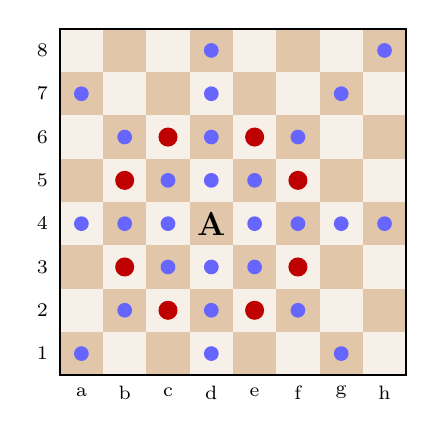
\begin{tikzpicture}[scale=0.55]
		\foreach \x in {0,...,7} \foreach \y in {0,...,7} {
			\pgfmathparse{mod(\x+\y,2)==0 ? "brown!45" : "brown!12"}
			\fill[\pgfmathresult] (\x,\y) rectangle ++(1,1);
		}
		\foreach \dx/\dy in {1/0,-1/0,0/1,0/-1,1/1,1/-1,-1/1,-1/-1} {
			\foreach \k in {1,...,7} {
				\pgfmathsetmacro{\px}{3+\k*\dx}\pgfmathsetmacro{\py}{3+\k*\dy}
				\ifdim \px pt>-1pt \ifdim \px pt<8pt \ifdim \py pt>-1pt \ifdim \py pt<8pt
					\fill[blue!60] (\px+0.5,\py+0.5) circle (0.17);
				\fi\fi\fi\fi
			}
		}
		\foreach \dx/\dy in {1/2,2/1,-1/2,-2/1,1/-2,2/-1,-1/-2,-2/-1} {
			\fill[red!75!black] (3+\dx+0.5,3+\dy+0.5) circle (0.22);
		}
		\node[font=\bfseries\large] at (3.5,3.5) {A};
		\draw[thick] (0,0) rectangle (8,8);
		\foreach \f [count=\i from 0] in {a,...,h} \node[font=\scriptsize] at (\i+0.5,-0.4) {\f};
		\foreach \r in {1,...,8} \node[font=\scriptsize] at (-0.4,\r-0.5) {\r};
	\end{tikzpicture}
	\caption{Az Amazon lépései a d4 mezőről: kék a vezérszerű , piros a huszárszerű célmezők.}
	\label{fig:amazonMoves}
\end{figure}

Az Amazon (\ref{fig:amazonMoves}.~ábra) üres táblán egy középső mezőről akár 35 mezőt is elérhet (27 vezérszerű + 8 huszárugrás), szemben a vezér 27 mezőjével. A huszárugrás az egyetlen olyan támadási forma, amelyet a vezér nem tud kivédeni közbeállással, ezért az Amazon egyedül is mattot adhat a magára hagyott királynak. Mivel a király ilyen bábu ellen különösen sebezhető, az Amazon jelentősen felülmúlja a vezért; a szakirodalom értékét általában 12--13 gyalogegységre teszi~\cite{ChessVariantsAmazon}. A motorban az Amazon a vezér helyén áll, és az ilyen változatban a vezér teljesen eltűnik a játékból: a gyalog is Amazonná változik a vezér helyett.

%----------------------------------------------------------------------------
\chapter{Előzmények és szakirodalmi háttér}\label{chap:background}
%----------------------------------------------------------------------------

\section{Táblareprezentáció}

A modern sakkmotorok túlnyomó többsége bitboardokkal írja le az állást~\cite{CPWBitboards}. A bitboard egy 64 bites egész szám, amelynek $i$-edik bitje azt jelzi, hogy az $i$-edik mezőn áll-e az adott típusú bábu. Bábutípusonként és színenként egy-egy bitboardot tárolva a lépésgenerálás és a támadásszámítás nagy része néhány bitművelettel (ÉS, VAGY, eltolás, \texttt{popcount}, legalacsonyabb bit keresése) elvégezhető, amelyeket a modern processzorok egyetlen utasítással hajtanak végre.

A csúszó bábuk (bástya, futó, vezér) támadásai a köztes mezők foglaltságától függenek. Erre a legelterjedtebb megoldás a magic bitboard technika~\cite{CPWMagic}: a releváns foglaltsági bitek egy előre megkeresett magic konstanssal szorozva és eltolva egy tömbindexet adnak, így a támadási halmaz egyetlen táblázat-kiolvasással megkapható.

Az állások gyors azonosítására a Zobrist-hash~\cite{Zobrist70} szolgál: minden (bábu, mező) párhoz, a lépésjoghoz, a sáncjogokhoz és az en passant oszlophoz egy-egy véletlen 64 bites számot rendelünk, és az állás kulcsa ezek XOR-ja. Lépéskor a kulcs inkrementálisan, néhány XOR-ral frissíthető. A kulcs az ismétlésfigyeléshez és a transzpozíciós táblához is használható.

A lépésgenerátor helyességét a perft (performance test) módszerrel szokás ellenőrizni: adott mélységig megszámoljuk az összes szabályos lépéssorozat végállását, és az eredményt ismert referenciaértékekkel vetjük össze~\cite{CPWPerft}.

\section{Keresés}

A kétszemélyes játékok klasszikus keresőeljárása a minimax, illetve ennek negamax alakja (amennyiben a két félnek a szabályai szimmetrikusak). Az alfa-béta vágás~\cite{Knuth75} ugyanazt az eredményt adja, mint a minimax, de jó lépésrendezés esetén a vizsgált csomópontok száma nagyjából a négyzetgyökére csökken. Erre az alapra épülnek a modern motorok további technikái:

\begin{itemize}
	\item \emph{Iteratív mélyítés:} a motor egyre nagyobb mélységgel keres, és az előző iteráció eredményét a lépésrendezéshez és az időkezeléshez használja.
	\item \emph{Transzpozíciós tábla (TT):} a már kiértékelt állások eredményét Zobrist-kulccsal indexelt hash-táblában tárolja~\cite{CPWTT}.
	\item \emph{Principal Variation Search (PVS):} a legjobbnak vélt lépés után a többit csak nulla szélességű ablakkal ellenőrzi.
	\item \emph{Nyugalmi keresés} (\emph{quiescence search}): a horizont-effektus elkerülésére a levélcsomópontokban az ütéseket tovább vizsgálja.
	\item \emph{Vágások és redukciók:} Null-Move pruning, Late Move reduction (LMR), futility, razoring jellegű vágások~\cite{CPWPruning}.
	\item \emph{Lépésrendezés:} TT-move, MVV-LVA, Static Exchange Evaluation (SEE), killer move, move history, counter move history.
	\item \emph{Párhuzamosítás:} a Lazy SMP eljárásban több szál keresi ugyanazt a fát, közös transzpozíciós táblán keresztül osztva meg az eredményeket~\cite{CPWLazySMP}.
\end{itemize}

\section{Állásértékelés: kézzel írt függvénytől az NNUE-ig}

Hagyományosan az állásértékelő függvény kézzel hangolt tagok összege: anyagérték, bábu-mező táblák, mobilitás, gyalogszerkezet, királybiztonság stb. 2018-ban Yu Nasu bemutatta az NNUE (Efficiently Updatable Neural Network) architektúrát~\cite{Nasu18}, amelyet 2020-ban a Stockfish is átvett. Az NNUE első rétege nagyon széles, de ritka bemenetű: a bemeneti jellemzők (például ,,saját király a g1-en, ellenséges huszár f6-on'') egy lépés hatására csak néhány helyen változnak, így az első réteg kimenete (az akkumulátor) lépésenként inkrementálisan frissíthető. Ettől lesz az értékelés elég gyors ahhoz, hogy a keresés minden csomópontjában használható legyen.

A motor két hálót is használ: a régebbi \emph{HalfKP} formátumú Stockfish-hálót a nyílt forrású \texttt{nnue-probe} könyvtáron~\cite{NnueProbe} keresztül, valamint egy újabb, \emph{HalfKAv2\_hm} formátumú hálót~\cite{NnuePytorch}.

\section{UCI protokoll}

A UCI~\cite{UCI} szöveges, soronkénti protokoll, amelyen keresztül egy grafikus felület (pl. Arena, Cute Chess, Lichess-bot) a motor standard bemenetére és kimenetére írva vezérli a motort. A legfontosabb parancsok: \texttt{uci} (azonosítás, válasz: \texttt{uciok}), \texttt{isready} (\texttt{readyok}), \texttt{ucinewgame}, \texttt{position startpos|fen \ldots{} moves \ldots}, \texttt{go} (paraméterei: \texttt{wtime}, \texttt{btime}, \texttt{winc}, \texttt{binc}, \texttt{movetime}), \texttt{stop} és \texttt{quit}. A motor a keresés végén \texttt{bestmove} sorral válaszol.

\section{Hasonló alkotások}

A legerősebb nyílt forrású motor a Stockfish~\cite{Stockfish}, amely a NNUE-t a fent vázolt keresési technikák igen kifinomult változataival kombinálja. Tündérsakk-változatok tekintetében a Fairy-Stockfish~\cite{FairyStockfish} a meghatározó: ez a Stockfish olyan elágazása, amely konfigurációs fájlból tetszőleges bábukat és szabályokat képes betölteni. Ennek a motor célja egy áttekinthető, mérésekkel alátámasztott, saját kódbázis volt, amelybe a tündérbábuk támogatása kis, jól körülhatárolt módosításokkal illeszthető.

%----------------------------------------------------------------------------
\chapter{Szoftverarchitektúra és UCI kommunikációs réteg}\label{chap:architecture}
%----------------------------------------------------------------------------

\section{Áttekintés}

A rendszer C++20 nyelven készült, és két tárolóban él. A backend egy konzolos projekt, amely a motort, a UCI-kiszolgálót és a robot-robot elleni mérőkörnyezetet tartalmazza. A GUI projekt ugyanazokat a motorforrásokat egy grafikus felülettel egészíti ki. A két tároló motorrésze forrásszinten megegyezik, így minden kereső- és lépésgenerátor-fejlesztés mindkét programban elérhető. A rétegeket \aref{fig:architecture}.~ábra mutatja.

\begin{figure}[!ht]
	\centering
	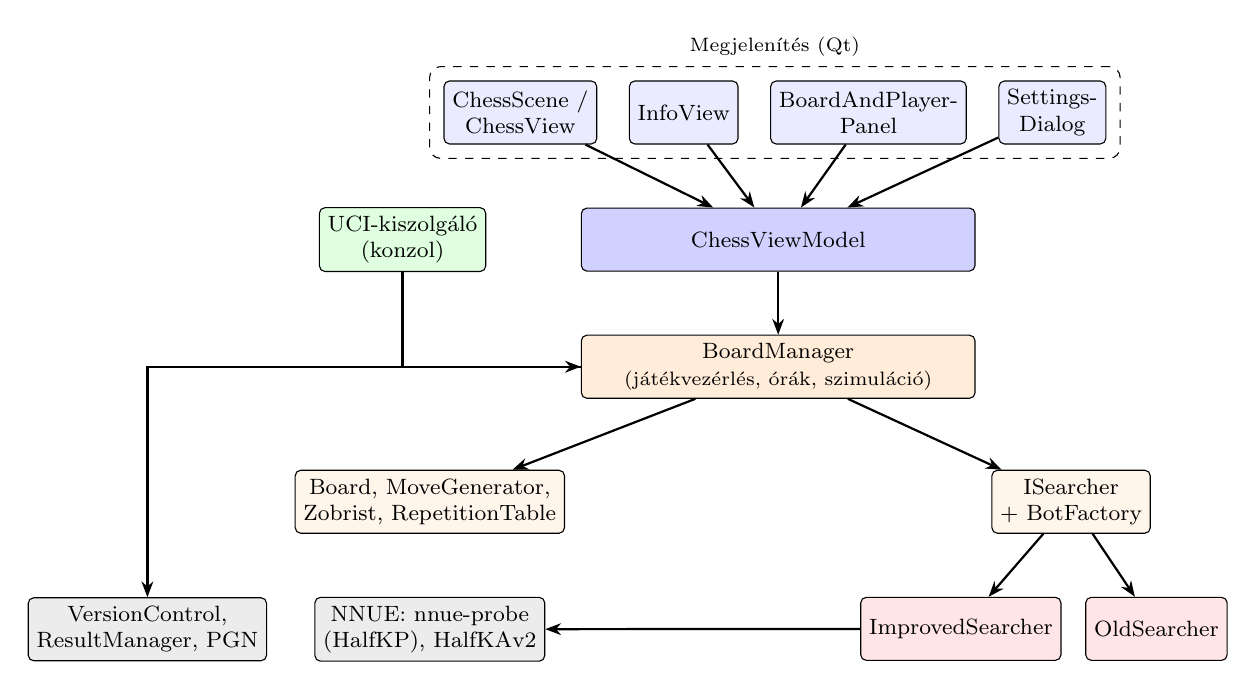
\begin{tikzpicture}[
		box/.style={draw, rounded corners=2pt, align=center, font=\footnotesize, minimum height=8mm, inner sep=3pt, fill=white},
		layer/.style={draw, dashed, rounded corners=4pt, inner sep=5pt},
		arr/.style={-{Stealth[length=2mm]}, thick}
	]
		\node[box, fill=blue!8] (scene) {ChessScene /\\ ChessView};
		\node[box, fill=blue!8, right=4mm of scene] (info) {InfoView};
		\node[box, fill=blue!8, right=4mm of info] (panel) {BoardAndPlayer-\\Panel};
		\node[box, fill=blue!8, right=4mm of panel] (settings) {Settings-\\Dialog};
		\node[box, fill=blue!18, below=8mm of info, xshift=12mm, minimum width=50mm] (vm) {ChessViewModel};
		\node[box, fill=green!12, left=12mm of vm] (uci) {UCI-kiszolgáló\\(konzol)};
		\node[box, fill=orange!15, below=8mm of vm, minimum width=50mm] (bm) {BoardManager\\{\scriptsize (játékvezérlés, órák, szimuláció)}};
		\node[box, fill=orange!8, below left=9mm and 2mm of bm] (board) {Board, MoveGenerator,\\Zobrist, RepetitionTable};
		\node[box, fill=orange!8, below right=9mm and 2mm of bm] (isearch) {ISearcher\\+ BotFactory};
		\node[box, fill=red!10, below=8mm of isearch, xshift=-14mm] (imp) {ImprovedSearcher};
		\node[box, fill=red!10, right=3mm of imp] (old) {OldSearcher};
		\node[box, fill=gray!15, below=8mm of board] (nnue) {NNUE: nnue-probe\\(HalfKP), HalfKAv2};
		\node[box, fill=gray!15, left=6mm of nnue] (util) {VersionControl,\\ResultManager, PGN};
		\begin{scope}[on background layer]
			\node[layer, fit=(scene)(settings), label={[font=\scriptsize]above:Megjelenítés (Qt)}] {};
		\end{scope}
		\draw[arr] (scene) -- (vm); \draw[arr] (info) -- (vm); \draw[arr] (panel) -- (vm); \draw[arr] (settings) -- (vm);
		\draw[arr] (vm) -- (bm); \draw[arr] (uci) |- (bm);
		\draw[arr] (bm) -- (board); \draw[arr] (bm) -- (isearch);
		\draw[arr] (isearch) -- (imp); \draw[arr] (isearch) -- (old);
		\draw[arr] (imp) -- (nnue); \draw[arr] (bm) -| (util);
	\end{tikzpicture}
	\caption{A rendszer rétegei. A kék elemek csak a GUI projektben, a zöld csak a konzolos backendben léteznek, a többi közös.}
	\label{fig:architecture}
\end{figure}

\section{Rétegek és felelősségek}

\begin{itemize}
	\item \textbf{Szabályréteg} (\texttt{Board}, \texttt{MoveGenerator}, \texttt{Zobrist}, \texttt{RepetitionTable}): az állás tárolása, a pszeudolegális lépések előállítása, a lépés végrehajtása és visszavonása, a sakk-, matt-, patt- és döntetlenfigyelés. Ez a réteg semmit sem tud a keresésről és a felületről.
	\item \textbf{Játékvezérlő} (\texttt{BoardManager}): egy játszma teljes állapotát kezeli: a sakkórákat, a robotok létrehozását és időbeállításait, a lépések visszavonását, a játszma végének felismerését, a megnyitáskönyvből indított robot-robot szimulációt és a UCI-hurkot.
	\item \textbf{Keresők} (\texttt{ISearcher} interfész): minden robot ugyanazt az interfészt valósítja meg (\texttt{setState}, \texttt{GetRobotMove}, \texttt{setDifficulty}, időkezelő függvények, \texttt{stopSearch}). A \texttt{BotFactory} típus alapján példányosítja az aktuális (\texttt{ImprovedSearcher}) vagy a referenciaként megtartott korábbi (\texttt{OldSearcher}) keresőt. A két kereső külön névtérben él, így egyszerre, egymás ellen is futtathatók.
	\item \textbf{Segédmodulok}: a \texttt{VersionControl} a keresők forráskódjáról SHA-256 lenyomatot készít, és minden új kódállapotot \texttt{vN} néven archivál; a \texttt{ResultManager} a robot-robot játszmák eredményét és PGN-jét verziópáronként menti; a \texttt{PGNFormatter} a lépéseket szabványos algebrai jelölésre (SAN) alakítja.
	\item \textbf{Megjelenítés} (csak GUI): MVVM jellegű felépítés, ahol a \texttt{ChessViewModel} közvetít a Qt-nézetek és a \texttt{BoardManager} között (részletesen \aref{chap:gui}.~fejezet).
\end{itemize}

A beállításokat egyszerű adatszerkezetek (\texttt{RobotSettings}, \texttt{BoardSettings}, \texttt{TimeSettings}, \texttt{VariantSettings}) hordozzák; ezek \texttt{operator!=} műveletével a nézetmodell pontosan eldönti, hogy egy változtatás új játszmát igényel-e, vagy elég a meglévőt frissíteni.

\section{Szálkezelés}

A keresés mindig külön szálon fut, hogy a felület és a sakkóra ne akadjon meg. A GUI a robot lépését QThread-ben számolja, és az eredményt sorba állított jelzéssel juttatja vissza a fő szálra; egy keresésazonosító biztosítja, hogy egy időközben megszakított (pl. visszavont) keresés eredménye ne kerüljön a táblára. Maga a kereső további segédszálakat indíthat (Lazy SMP, \aref{sec:lazysmp}.~szakasz). A tömeges robot-robot szimuláció során minden szál saját \texttt{BoardManager} példánnyal és saját robotokkal dolgozik, csak a statisztika összesítése és a konzolkimenet közös, mutex-szel védve.

\section{Verziókezelés és mérési infrastruktúra}\label{sec:versioning}

A fejlesztés egyik legfontosabb eszköze az automatikus verziózás volt. Robot-robot szimuláció indításakor a \texttt{VersionControl} kiszámítja mindkét kereső forráskönyvtárának hash-ét, ha ilyen kódállapot még nem volt, a forrásokat \texttt{generatedBotVersions/<kereső>/vN/src} alá másolja. Az eredmények \texttt{botvsbotresults/<kereső1>-<kereső2>/<kereső1\_vN>-<kereső2\_vM>/} mappába kerülnek: a \texttt{results.txt} az összesített győzelem/döntetlen/vereség számokat, a \texttt{Matches} alkönyvtár pedig eredmény szerint csoportosítva minden játszma PGN-jét tartalmazza. Így minden mérés utólag is visszakereshető és megismételhető.

A szimuláció a 22\,234 különböző állást tartalmazó megnyitáskönyvből (assets/openings.txt) véletlenszerű kezdőállást választ, és minden kezdőállásból két játszmát játszat, színcserével. Ez kiszűri a megnyitásválasztásból és a világos kezdés előnyéből adódó torzítást.

\section{A UCI kommunikációs réteg}\label{sec:uci}

A konzolos program UCI-kiszolgálóként indul (\texttt{BoardManager::runUCIService}). A szöveges parancsokat soronként olvassa, és az első szó alapján dolgozza fel; a lépések UCI-formátumú (pl. \texttt{e7e8q}) szövegét a \texttt{UCIParsing} alakítja belső lépéssé és vissza. A \texttt{go} parancs fix idős (\texttt{movetime}) és órás (\texttt{wtime}/\texttt{btime}/\texttt{winc}/\texttt{binc}) módot is ismer; ez utóbbit a robot időkezelője (\aref{sec:time}.~szakasz) használja fel. Egy rövid, valódi munkamenet:

\begin{lstlisting}[caption={UCI munkamenet (bemenet és a motor válaszai)}, label={lst:uci}]
> uci                                   < id name <bot's name>
                                        < id author <name>
                                        < uciok
> isready                               < readyok
> position startpos moves e2e4 e7e5
> go movetime 1000                      < bestmove g1f3
> position fen 6k1/5ppp/8/8/8/8/5PPP/3Q2K1 w - - 0 1
> go movetime 500                       < bestmove d1d8
\end{lstlisting}

A protokollnak köszönhetően a motor bármely UCI-kompatibilis felületről (pl. Cute Chess, általam haszsnált környezet) használható, és más motorok ellen is versenyeztethető.

%----------------------------------------------------------------------------
\chapter{Táblareprezentáció és lépésgenerálás}\label{chap:movegen}
%----------------------------------------------------------------------------

\section{Az állás tárolása}

A \texttt{Board} osztály az állást színenként és bábutípusonként egy-egy 64 bites bitboardban tárolja (m\_bitboards[2][PIECE\_TYPE\_COUNT]); a mezők számozása a1~=~0-tól h8~=~63-ig halad. Ezek mellett színenként egy foglaltsági bitboard és egy összesített foglaltság is rendelkezésre áll, amelyeket minden lépés inkrementálisan frissít. A nem bitboard jellegű állapotot (sáncjogok, en passant mező, ütött bábu típusa, félléptetés-számláló, lépésszám, Zobrist-kulcs) egy kompakt \texttt{BoardState} rekord tárolja, és ezekből egy 1024 elemű tömb őrzi a teljes előzményt. Így a lépés visszavonásához nem kell semmit újraszámolni, csak az előző rekordra visszalépni.

\section{A lépés kódolása}

Egy lépés (\texttt{Move}) 16 bitbe tömörítve tárolja a kiinduló mezőt (6 bit), a célmezőt (6 bit) és egy 4 bites jelzőt, mellette egy bájton a mozgó bábu típusát. A jelzőbitek külön-külön kódolják az ütést és az átváltozást, a maradék két bit pedig a lépés altípusát: dupla gyaloglépés, rövid vagy hosszú sánc, en passant, illetve átváltozásnál a választott bábut (huszár, futó, bástya, vezér). A tömör forma miatt egy lépés egyetlen gépi szóban mozgatható, és a transzpozíciós tábla bejegyzésébe is belefér. A lépéslista (\texttt{MoveList}) egy 256 elemű, rögzített méretű tömb: a keresés során így egyáltalán nincs dinamikus memóriafoglalás.

\section{Támadási táblák és mágikus bitboardok}

A program indulásakor egyszer (\texttt{std::call\_once}) épülnek fel az előre kiszámított táblák:
\begin{itemize}
	\item a huszár, a király és a gyalogok (színenként) támadási halmaza mind a 64 mezőre,
	\item a bástyák ($64\times4096$) és futók ($64\times512$) mágikus bitboard-táblái, előre megkeresett mágikus konstansokkal és eltolásokkal,
	\item a szabad gyalog maszkok, amelyeket a kézzel írt értékelés és a keresés is használ.
\end{itemize}
Egy csúszó bábu támadásainak lekérdezése így egy maszkolás, egy szorzás, egy eltolás és egy táblaolvasás; a vezér támadása a bástya- és a futótámadás uniója.

\section{Pszeudolegális generálás és legalitásvizsgálat}

A \texttt{MoveGenerator} a lépő fél minden bábujára előállítja a pszeudolegális lépéseket, vagyis azokat, amelyek a bábu mozgásszabályainak megfelelnek, de esetleg sakkban hagyják a saját királyt. A sáncolásnál a generátor már itt ellenőrzi, hogy a király nem áll sakkban, és nem halad át megtámadott mezőn. A nyugalmi kereséshez létezik egy csak ütéseket előállító mód is.

A legalitás eldöntése a \texttt{MakeMove} feladata: a lépés végrehajtása után megvizsgálja, hogy a lépő fél királyát támadja-e valami (isSquareAttacked), és ha igen, a lépést azonnal visszavonja és elutasítja. A támadásvizsgálat fordított irányban dolgozik: a király mezőjéről indítja a huszár-, király-, gyalog- és csúszótámadásokat, és ezek metszetét képezi az ellenfél megfelelő bitboardjaival. Ez a megközelítés egyszerűbb a teljesen legális generálásnál, és a keresésben nem drágább, mert a lépések jelentős része a vágások miatt végre sem hajtódik.

A lépés végrehajtásakor a sáncjogok frissítéséhez egy mezőnkénti maszk (castling\_mask) elég: ha egy lépés a király vagy egy bástya kiinduló mezőjét érinti, a megfelelő jog egyetlen ÉS művelettel törlődik. A Zobrist-kulcsot a \texttt{MakeMove} inkrementálisan, XOR-okkal frissíti, a GenerateFullHash csak a FEN betöltésekor számol teljes kulcsot, mivel ez egy lassú művelet. A \texttt{MakeMove} kétféle módban hívható: keresési módban csak a fenti minimális munkát végzi, játszma módban (a felület és a játékvezérlő számára) eltárolja a lépést, a táblaképet, a sakkjelzést és a következő állás szabályos lépéseit is, amelyekből a lépéslista, a SAN-jelölés és a visszajátszás dolgozik.

\section{Döntetlenek és ismétlésfigyelés}

A \texttt{RepetitionTable} a játszma és a keresés során előforduló állások kulcsait tárolja. Mivel ütés vagy gyaloglépés után korábbi állás már nem ismétlődhet meg, minden ilyen visszafordíthatatlan lépés új ablakot nyit, és az ismétlést csak az aktuális ablakban kell keresni. A játszmában a háromszori ismétlés a döntetlen, a keresésben viszont már a kétszeri is annak számít: ha egy állás egyszer már előfordult, a motor az ismétlésre vezető ágat döntetlenként értékeli, így felesleges mélységet takarít meg. Ezen felül a tábla az ötvenlépéses szabályt (100 féllépés) és az elégtelen anyagot is felismeri (csak királyok, király és egy könnyűtiszt, azonos színű futók).

A lépésgenerátor helyességét és sebességét \aref{sec:perft}.~szakasz perft-mérései igazolják.

%----------------------------------------------------------------------------
\chapter{A keresőmotor}\label{chap:search}
%----------------------------------------------------------------------------

A motor agya az \texttt{ImprovedSearcher} névtér \texttt{Searcher} osztálya. Ez a fejezet a kereső minden funkcióját bemutatja. A zárójelben szereplő \textbf{vN} jelzés azt a verziót adja meg, amelyben az adott technika először megjelent, a hozzá tartozó mérést \aref{sec:versions}.~szakasz tartalmazza. A kereső a v1-ben szándékosan egy minimális magról (alfa-béta, NNUE, nyugalmi keresés) indult, és minden további elem külön verzióként, mérve került bele.

\section{A keresés kerete}

\paragraph{Iteratív mélyítés (v1).} A kereső 1-es mélységtől kezdve egyre mélyebben keres, amíg az időkezelő meg nem állítja. Minden befejezett iteráció legjobb lépése és értéke megmarad, így egy félbeszakított iteráció sem okoz rossz döntést, az előző iteráció eredménye pedig a következő lépésrendezését és ablakát segíti.

\paragraph{Negamax alfa-béta, fail-soft (v4, teljesen v23).} A rekurzív negamax a szokásos alfa-béta vágással dolgozik. A fail-soft változat az ablakon kívül eső értékeket is a lehető legpontosabban adja vissza, ami a transzpozíciós tábla bejegyzéseit és az aspirációs ablak újrakeresését is pontosabbá teszi.

\paragraph{Principal Variation Search (v7).} Egy csomópont első (legjobbnak vélt) lépését teljes ablakkal, a többit nulla szélességű ablakkal ($[\alpha, \alpha+1]$) keresi. Ha egy későbbi lépés mégis jobbnak bizonyul, teljes ablakkal újrakeresi. Jó lépésrendezés esetén a nulla ablakos keresések sokkal olcsóbbak.

\paragraph{Aspirációs ablak (v14, mai formája v23).} 4-es mélységtől a gyökérkeresés nem $(-\infty, +\infty)$ ablakkal indul, hanem az előző iteráció értéke körüli $\pm\delta$ ablakkal, ahol $\delta = 25 + |s|/8$ centigyalog. Ha az eredmény az ablakon kívül esik, a kereső a megfelelő irányban duplázza az ablakot, és újrakeres.

\paragraph{Gyökérlépés-rendezés és főváltozat (v17).} A gyökérben a lépéseket az előző iteráció pontszáma szerint rendezi. A főváltozatot (PV) egy  PV-tábla gyűjti, amelyet a BuildPvString a transzpozíciós táblából legális lépésekkel tovább bővít, ez jelenik meg az info kimenetben.

\paragraph{Matt-távolság vágás és döntetlenek (v1).} Ha már egy rövidebb matt ismert, az ennél hosszabb mattot kereső ágak azonnal levághatók. A keresés minden csomópontban ellenőrzi az ötvenlépéses szabályt, az elégtelen anyagot és az ismétlést; a fán belül már a kétszeri ismétlés is döntetlen (\aref{chap:movegen}.~fejezet).

\section{Transzpozíciós tábla (v3, klaszterek v13, zármentes v23)}

A transzpozíciós tábla (TT) 128~MB méretű, kettő hatványa számú, 64 bájtra igazított klaszterből áll. Egy klaszter négy 16 bájtos bejegyzést tartalmaz, így egy lekérdezés egyetlen gyorsítótár-sort érint. A bejegyzés egy 64 bites kulcsot és egy 64 bites, tömörített adatot tárol: érték (16 bit), lépés (16 bit), bábutípus, mélység, korlát típusa (pontos, alsó vagy felső korlát) és generáció (8--8 bit).

A többszálú kereséshez a tábla zármentes: a kulcs helyett a kulcs XOR adat értéket tárolja. Ha két szál egyszerre írja ugyanazt a bejegyzést, és az olvasó egy félig frissített állapotot lát, a XOR-ellenőrzés nem egyezik, és a bejegyzés egyszerűen érvénytelennek számít. Ez lényegesen gyorsabb a korábbi (v16--v20) mutex-, illetve spinlock-alapú megoldásnál.

A csere sorrendje: üres hely, azonos kulcsú bejegyzés, végül a legkisebb ,,$4\cdot\text{kor} - \text{mélység}$'' értékű bejegyzés. A matt-értékeket a tárolás a gyökértől mért távolságra korrigálja. TT-vágás csak nem-PV csomópontban történik, és nem, ha a félléptetés-számláló már 90 felett van (az ötvenlépéses szabály közelében a tárolt érték félrevezető lehet). A tábla a következő csomópont klaszterét előre betölti (prefetch), mielőtt a lépést végrehajtaná.

\section{Lépésrendezés}

Az alfa-béta hatékonysága szinte teljesen a lépésrendezésen múlik. A lépéseket a kereső pontozza (\aref{tab:ordering}.~táblázat), majd nem rendezi az egész listát, hanem mindig csak a következő legjobbat választja ki (lazy pick-best, v17), mert egy vágás után a többi lépést úgysem kell megvizsgálni.

\begin{table}[!ht]
	\footnotesize
	\centering
	\begin{tabular}{l r l}
		\toprule
		Lépés típusa & Pontszám & Verzió \\
		\midrule
		TT-lépés & 10\,000\,000 & v3 \\
		Ütés vezérré/Amazonná vagy huszárrá változással & 9\,000\,000 / 8\,000\,000 & v12 \\
		Nem vesztes ütés (MVV-LVA, SEE $\ge 0$) & $5\,000\,000 + 16\cdot\text{áldozat} - \text{támadó}$ & v1/v12 \\
		Csendes átváltozás vezérré/Amazonná vagy huszárrá & 4\,000\,000 / 3\,000\,000 & v12 \\
		1. és 2. gyilkos lépés & 2\,000\,000 / 1\,500\,000 & v5 \\
		Ellenlépés (countermove) & 1\,200\,000 & v6 \\
		Csendes lépés & történeti érték & v6 \\
		Vesztes ütés (SEE $<0$) & $-1\,000\,000$ & v12 \\
		Bástyává/futóvá alulátváltozás & $-2\,000\,000$ & v12 \\
		\bottomrule
	\end{tabular}
	\caption{A lépések rendezési pontszámai.}
	\label{tab:ordering}
\end{table}

\paragraph{MVV-LVA és SEE.} Az ütéseket elsősorban az ütött bábu értéke, másodsorban az ütő bábu olcsósága szerint rendezi (Most Valuable Victim -- Least Valuable Attacker). Ha az ütő értékesebb az áldozatnál, a statikus cserekiértékelés (SEE)~\cite{CPWSEE} dönti el, hogy a cserelánc a végén nyereséges-e: a mező összes támadóját a legolcsóbbtól kezdve felváltva üti le, a röntgentámadásokat (pl. bástya a bástya mögött) is figyelembe véve.

\paragraph{Gyilkos lépések (v5) és ellenlépés (v6).} Egy csendes lépés, amely egy testvércsomópontban vágást okozott, valószínűleg itt is jó: ezt féllépésenként két gyilkos lépés tárolja. Az ellenlépés-heurisztika az ellenfél előző lépésére (bábutípus és célmező) adott legjobb választ jegyzi meg.

\paragraph{Történeti heurisztika (v6, gravitáció v18).} Minden csendes lépés (szín, honnan, hová) kap egy pontszámot, amely vágás esetén nő, a vágás előtt kipróbált, sikertelen csendes lépéseknél pedig csökken. A gravitációs frissítés a pontszámot korlátok között tartja, így a régi információ fokozatosan elévül.

\section{Vágások, redukciók és kiterjesztések}

\Aref{tab:pruning}.~táblázat a végleges kereső összes vágási és redukciós technikáját foglalja össze; a feltételek a nem-PV csomópontokra vonatkoznak, ha nincs sakk.

\begin{table}[!ht]
	\scriptsize
	\centering
	\begin{tabularx}{\linewidth}{l X l}
		\toprule
		Technika & Működés (végleges paraméterek) & Verzió \\
		\midrule
		Fordított futility & ha $\text{eval} - (100d - 75\cdot\text{javuló}) \ge \beta$ és $d \le 6$, a csomópont azonnal elvágható & v9 \\
		Razoring & ha $d \le 3$ és $\text{eval} + 200 + 150d < \alpha$, csak nyugalmi keresés dönt & v9 \\
		Null-lépés vágás & a lépésjogot átadva, $R = (823 + 67d)/256 + \min((\text{eval}-\beta)/200, 3)$ redukcióval keres; ha az ellenfél így sem éri el $\beta$-t, vágás; gyalogvégjátékban tiltott (zugzwang) & v8 \\
		Futility vágás & $d \le 6$ esetén a csendes lépések kihagyása, ha $\text{eval} + 120d \le \alpha$ & v10 \\
		Késői lépések vágása & $(\text{javuló} ? 4 : 2) + d^2$ csendes lépés után a többi kihagyása, $d \le 8$ & v11 \\
		SEE-vágás & $d \le 7$ esetén a $-50d$ (csendes) vagy $-90d$ (ütés) alatti SEE-jű lépések kihagyása & v11 \\
		LMR & a késői, csendes lépések csökkentett mélységű keresése (lásd lent) & v7 \\
		IIR & TT-lépés hiányában a mélység eggyel csökken & v23 \\
		Szinguláris kiterjesztés & ha a TT-lépés minden más lépésnél jelentősen jobb, $+1$ mélység; több vágó alternatíva esetén ,,multi-cut'' vágás vagy $-1$ kiterjesztés & v23 \\
		\bottomrule
	\end{tabularx}
	\caption{Vágások, redukciók és kiterjesztések ($d$: hátralévő mélység, eval: statikus értékelés).}
	\label{tab:pruning}
\end{table}

\paragraph{A javulás jelző (v9).} Ha a lépő fél statikus értékelése jobb, mint két félléptetéssel korábban, az állás javuló. Ilyenkor a kereső óvatosabban vág (nagyobb futility-ráhagyás, több lépés a késői lépések vágása előtt, kisebb LMR-redukció), hiszen az állás valószínűleg még tartogat valamit.

\paragraph{Késői lépések redukciója (v7, külön PV-tábla v11).} A rendezés végén álló csendes lépések nagy valószínűséggel rosszak, ezért a kereső csökkentett mélységgel vizsgálja őket, és csak akkor keresi újra teljes mélységgel, ha meglepően jónak bizonyulnak. Az alapredukció egy előre kiszámított táblából jön: nem-PV csomópontban $0{,}5 + \ln d \cdot \ln m / 2{,}5$, PV-ben $-0{,}25 + \ln d \cdot \ln m / 3$, ahol $m$ a lépés sorszáma. Ezt módosítja, hogy javuló-e az állás, gyilkos lépésről, szabad gyalog előretolásáról, sakkadásról, átváltozásról van-e szó, illetve a lépés történeti pontszáma ($\pm2$).

\paragraph{Szinguláris kiterjesztés (v23).} Ha 8-as mélység felett a TT-lépés értéke megbízható, a kereső a TT-lépés kihagyásával, csökkentett mélységgel és $\text{TT-érték} - (3 + d/2)$ korláttal ellenőrzi a többi lépést. Ha egyik sem éri el ezt, a TT-lépés az egyetlen jó lépés, ezért egy mélységgel tovább keresi; ha viszont már a korlát is vágást okoz, több jó lépés van, és a csomópont azonnal levágható.

\paragraph{Sakk-kiterjesztés.} A korai verziók minden sakkadást egy mélységgel meghosszabbítottak. A v23 ezt kivette, mert a szinguláris kiterjesztés és a nyugalmi keresés a fontos sakkokat már lefedi, a kiterjesztés pedig a mérésekben inkább rontott.

\section{Nyugalmi keresés (v1)}

A mélységkorlát elérésekor a kereső nem azonnal értékel, hanem csak az ütéseket (és az erős átváltozásokat) vizsgálja tovább, amíg az állás nyugodt nem lesz. A lépő fél állva maradhat: ha a statikus értékelés már eléri $\beta$-t, nem kell tovább keresni. A végleges változat elemei: kitérő lépések generálása sakkban (v2--v3), delta-vágás (v3; kihagyja azt az ütést, amely még a legnagyobb lehetséges nyereséggel sem érné el $\alpha$-t), SEE-vágás (v11), TT-lekérdezés és -tárolás (v23), valamint a bástyává és futóvá alakuló átváltozások elhagyása.

\section{Állásértékelés}

\paragraph{NNUE HalfKP (v1).} A kezdeti értékelés a Stockfish egy HalfKP formátumú hálója (\texttt{nn-62ef826d1a6d.nnue}) a \texttt{nnue-probe} könyvtáron keresztül. A kereső minden lépésnél csak a megváltozott bábukat (dirty pieces: mozgó bábu, ütött bábu, sáncnál a bástya, átváltozásnál a gyalog és az új bábu) adja át, a könyvtár ezekből inkrementálisan frissíti az akkumulátort.

\paragraph{NNUE HalfKAv2\_hm (v23).} A legfrissebb verzió egy újabb generációs, HalfKAv2\_hm formátumú Stockfish-hálót (nn-dabb1ed23026.nnue) használ, amelynek kiértékelését saját kóddal valósítottam meg (nnue-halfkav2). A háló $22\,528$ bemeneti jellemzőt (király helye $\times$ bábu $\times$ mező, a király oldalára tükrözve), $2\times1024$ neuronos első réteget, 8 anyagi vödröt és vödrönként külön 15--32--1 neuronos réteghalmazt tartalmaz. A vödröt a táblán lévő bábuk száma választja ki, így a háló külön réteget használ a megnyitásra, a középjátékra és a végjátékra. Az akkumulátorok egy veremben, félléptetésenként inkrementálisan frissülnek, ha valamelyik király mozog, az adott nézőpont akkumulátorát a kód teljesen újraszámolja. A belső szorzások AVX2 utasításokkal futnak.

\paragraph{Kézzel írt értékelés.} A gyengébb nehézségi szintek egy saját, kézzel hangolt értékelőt használnak: anyag és bábu-mező táblák középjátékra és végjátékra külön, játékfázis szerinti átmenettel, mobilitás, gyalogszerkezet (szabad, elszigetelt gyalogok), királybiztonság és gyalogpajzs, bábuegyensúly, ismert döntetlen végjátékok felismerése és a mop-up tag, amely nyert végjátékban a vesztes királyt a szélre szorítja. Ez gyengébb, mint az NNUE, de pont ez a cél: emberibb, hibázó játékot ad.

\section{Időkezelés}\label{sec:time}

Fix idős módban a kereső a megadott ideig gondolkodik. Órás módban két határt számol: a puha határ $\text{hátralévő idő}/40 + 0{,}8\cdot\text{bónusz}$, a kemény határ ennek háromszorosa (mindkettő a hátralévő időhöz korlátozva). Új iterációt csak a puha határ előtt kezd; ha a legjobb lépés háromszor egymás után nem változott, a puha határ 60\%-ánál is megáll. Válság esetén, ha az érték 50 centigyalognál többet esett, de az állás még nem dőlt el ($\pm800$ centigyalogon belül), a puha határon túl is folytatja, a kemény határ 80\%-áig.

\section{Többszálú keresés: Lazy SMP (v16)}\label{sec:lazysmp}

A kereső a beállított számú szálon fut. A segédszálak ugyanazt az állást keresik, saját előzménytáblával és lépésrendezéssel, de közös transzpozíciós táblán keresztül. Mivel a szálak kissé eltérő sorrendben haladnak, egymás számára hasznos TT-bejegyzéseket hagynak hátra, így a fő szál gyorsabban ér el egy adott mélységet. A szálak egy közös megállító jelzőn keresztül állnak le, az eredményt mindig a fő szál adja.

\section{Nehézségi szintek}

A négy nehézségi szint (\aref{tab:difficulty}.~táblázat) nem egyszerűen a keresési mélységet korlátozza. Az alsó három szint kézzel írt értékelést használ, és a \texttt{GetBestAmongTopMoves} egy több jelöltlépést kiértékelő keresés után szándékos hibát is véthet: adott valószínűséggel a legjobb $N$ lépés közül választ egy olyat, amely legfeljebb a küszöbnyit rosszabb a legjobbnál. A Haladó és Nehéz szint kiszűri a kínos hibákat (amikor a választott lépés után egy bábu védtelenül üthetővé válik), és egy ingyen kínálkozó bábut mindig leüt. Két szándékos hiba között legalább egy-két normál lépést tesz.

\begin{table}[!ht]
	\footnotesize
	\centering
	\begin{tabular}{l c c c c c c}
		\toprule
		Szint & Max. mélység & Értékelés & Hiba esélye & Top $N$ & Küszöb [cp] & Kínos hiba szűrése \\
		\midrule
		Kezdő & 6 & kézzel írt & 40\% & bármelyik & 900 & nem \\
		Haladó & 6 & kézzel írt & 30\% & 10 & 500 & igen \\
		Nehéz & 9 & kézzel írt & 20\% & 8 & 300 & igen \\
		Mester & -- & NNUE & 0\% & -- & -- & -- \\
		\bottomrule
	\end{tabular}
	\caption{A nehézségi szintek paraméterei (\texttt{SearcherSettings}).}
	\label{tab:difficulty}
\end{table}

%----------------------------------------------------------------------------
\chapter{A grafikus felhasználói felület}\label{chap:gui}
%----------------------------------------------------------------------------

\section{Felépítés}

A felület Qt~6-ban készült, a táblát a Qt Graphics View keretrendszere~\cite{QtGraphicsView} rajzolja. A szerkezet a Model--View--ViewModel mintát követi:
\begin{itemize}
	\item a \emph{modell} a \texttt{BoardManager} és a motor (\aref{chap:architecture}.~fejezet),
	\item a \emph{nézetmodell} a \texttt{ChessViewModel}: lefordítja a felhasználói műveleteket (lépés, visszavonás, feladás, új játszma, beállítások) motorhívásokká, kezeli a robot keresőszálát és a sakkórák időzítőjét, és Qt-jelzésekkel (\texttt{boardChanged}, \texttt{moveMade}, \texttt{gameEnded}, \ldots) értesíti a nézeteket,
	\item a \emph{nézetek}: a táblát rajzoló \texttt{ChessScene}/\texttt{ChessView}, a lépéslistát és a vezérlőgombokat tartalmazó \texttt{InfoView}, a játékosok adatait, óráit és a leütött bábukat mutató \texttt{BoardAndPlayerPanel}, valamint a \texttt{SettingsDialog}.
\end{itemize}
A nézetek soha nem érik el közvetlenül a motort, így a tábla rajzolása és a keresés egymástól teljesen független.

\begin{figure}[H]
	\centering
	\screenshot{gui_main_start.png}{A teljes főablak a kezdőállásban: tábla, játékospanelek, lépéslista, gombok.}{width=150mm,keepaspectratio}
	\caption{A program főablaka.}
	\label{fig:guiMain}
\end{figure}

\section{A főablak}

\Aref{fig:guiMain}.~ábrán látható főablak bal oldalán a tábla, felette és alatta a két játékos panelje áll. A panel a játékos nevét (robot esetén a kereső nevét és nehézségi szintjét), ikonját, a sakkórát, a leütött ellenséges bábukat és az anyagi előnyt (pl. ,,+3'') mutatja. A jobb oldali információs panelen a játszma lépései SAN-jelöléssel, a mozgó bábu ikonjával jelennek meg. A lépéslista alatt navigációs gombokkal (\guillemotleft, \guilsinglleft, \guilsinglright, \guillemotright) vagy egy lépésre kattintva a játszma bármely korábbi állása visszanézhető; ilyenkor a tábla és az órák a régi állapotot mutatják. Az ,,Új Játék'', ,,Visszavonás'' és ,,Feladás'' gombok, valamint a fogaskerék ikonú beállítások gomb zárják a panelt. A játszma végén a panel az eredményt (pl. ,,1 -- 0, Világos nyert'') is kiírja.

\section{Interakció a táblán}

A bábuk egérrel húzhatók (drag and drop), vagy kattintással kijelölhetők, majd a célmezőre kattintva léptethetők. Kijelöléskor a felület pontokkal jelöli a szabályos célmezőket (ez kikapcsolható), kiemeli a legutóbbi lépés két mezőjét, sakk esetén pirossal a megtámadott királyt, és az egér alatti mezőt is. A szabályos lépések listáját a motor számolja, a felület csak megjeleníti, így a felület soha nem enged szabálytalan lépést. Átváltozáskor a célmező oszlopában négy választható bábu jelenik meg (\ref{fig:guiPlay}.~ábra). Robot ellen játszva a robot a felhasználó lépése után automatikusan, külön szálon gondolkodik, ha a felhasználó közben visszavon vagy új játszmát indít, a keresés megszakad.

\begin{figure}[H]
	\centering
	\screenshot{gui_midgame_legal.png}{Középjáték: kijelölt bábu a szabályos célmezőkkel, kiemelt utolsó lépés, leütött bábuk és anyagi előny a panelen.}{width=115mm,keepaspectratio}\\[4mm]
	\screenshot{gui_promotion.png}{Gyalogátváltozás: a négy választható bábu a célmező oszlopában.}{width=115mm,keepaspectratio}
	\caption{Lépés közben megjelenített segítségek (fent) és az átváltozás bábuválasztója (lent).}
	\label{fig:guiPlay}
\end{figure}

\section{Beállítások}

A beállítások ablak négy fülön csoportosítja a lehetőségeket (\ref{fig:guiSettings}.~ábra):
\begin{itemize}
	\item \emph{Robotok:} külön-külön beállítható, hogy világos és/vagy sötét robot legyen, és milyen nehézségi szinten (Kezdő, Haladó, Nehéz, Mester) játsszon; itt kapcsolható be a robot-robot mód és állítható a robot maximális gondolkodási ideje.
	\item \emph{Tábla:} tábla megfordítása, a szabályos lépések jelölése és tetszőleges kezdőállás megadása FEN-ben.
	\item \emph{Időkontroll:} óra nélküli vagy ,,torna'' mód, a két fél alapideje külön-külön, és a lépésenkénti bónuszidő.
	\item \emph{Változatok:} a játékváltozat (Normál vagy Amazon sakk) kiválasztása (\aref{chap:amazon}.~fejezet).
\end{itemize}
A dialógus csak a ,,Mentés'' gombra írja vissza az értékeket; a nézetmodell ezután összeveti a régi és új beállításokat, és csak akkor indít új játszmát, ha erre szükség van (pl. megváltozott a kezdőállás vagy a robot típusa).

\begin{figure}[H]
	\centering
	\screenshot{gui_settings_robots.png}{Beállítások -- Robotok fül.}{width=72mm,keepaspectratio}\hspace{4mm}
	\screenshot{gui_settings_board.png}{Beállítások -- Tábla fül.}{width=72mm,keepaspectratio}\\[4mm]
	\screenshot{gui_settings_time.png}{Beállítások -- Időkontroll fül, ,,Torna mód'' kiválasztva.}{width=72mm,keepaspectratio}\hspace{4mm}
	\screenshot{gui_settings_variant.png}{Beállítások -- Változatok fül, ,,Amazon sakk'' kiválasztva.}{width=72mm,keepaspectratio}
	\caption{A beállítások ablak négy füle.}
	\label{fig:guiSettings}
\end{figure}

\section{Játék sakkórával és robot-robot mód}

Torna módban mindkét fél órája a beállított alapidőről indul, a lépő fél órája másodpercenként frissül, lépés után pedig a bónuszidővel nő. Az órák állását a játékvezérlő minden félléptetés után elmenti, így visszavonáskor az órák is visszaállnak. Robot-robot módban a felület a megnyitáskönyvből véletlen kezdőállást választ, és a két kereső egymás ellen játszik, színcserés párokban; ez a mód a fejlesztés során a motor viselkedésének szemmel követésére szolgált (\ref{fig:guiClock}.~ábra).

\begin{figure}[H]
	\centering
	\screenshot{gui_tournament_clock.png}{Torna módú játszma robot ellen, mindkét óra látszik, az egyik aktív.}{width=115mm,keepaspectratio}\\[4mm]
	\screenshot{gui_game_over.png}{Befejezett játszma: matt, az eredmény a jobb oldali panelen.}{width=115mm,keepaspectratio}
	\caption{Sakkórás játszma robot ellen (fent) és egy befejezett játszma eredménykijelzése (lent).}
	\label{fig:guiClock}
\end{figure}

%----------------------------------------------------------------------------
\chapter{Tündérsakk-kiterjesztés: az Amazon sakk}\label{chap:amazon}
%----------------------------------------------------------------------------

\section{A változat szabályai}

Az ,,Amazon sakk'' változatban mindkét fél vezérének helyén (d1, d8) egy Amazon áll, amely vezérként és huszárként is léphet (\aref{fig:amazonMoves}.~ábra). A változatban vezér egyáltalán nincs: a gyalog átváltozáskor huszárrá, futóvá, bástyává vagy Amazonná változhat. Minden más szabály (sáncolás, en passant, döntetlenek) változatlan. A kezdőállás FEN-jelöléssel \texttt{rnbakbnr/pppppppp/8/8/8/8/PPPPPPPP/RNBAKBNR w KQkq - 0 1}, ahol az Amazon jele \texttt{A}, illetve \texttt{a}.

\section{Megvalósítás a motorban}

A kiterjesztés célja az volt, hogy a meglévő kódhoz minél kevesebb, jól körülhatárolt módosítással illeszkedjen.

\paragraph{Bábutípus és állapot.} Az \texttt{AMAZON} új bábutípusként a \texttt{KING} után került a felsorolásba. Így a korábbi típusok indexei (és minden rájuk épülő tábla, pl. bábu-mező táblák) változatlanok maradtak, a bitboard-tömb és a Zobrist-kulcsok tömbje pedig automatikusan eggyel nőtt. Az összes ,,minden bábutípuson'' végigmenő ciklus a \texttt{PIECE\_TYPE\_COUNT} határig fut, így a FEN-olvasás és -írás, a hash-számítás és a táblakép is kezeli az új bábut.

\paragraph{Lépésgenerálás és támadásszámítás.} Az Amazon célmezői a bástya-, futó- és huszártámadások uniója. Mivel a sakkfigyelés fordított irányú (\aref{chap:movegen}.~fejezet), elég volt az Amazon bitboardját a huszár- és mindkét csúszótámadás ellenőrzéséhez hozzáadni. Ugyanígy bővült a cserekiértékeléshez (SEE) használt \texttt{getAttacksTo}, a röntgentámadásokat adó \texttt{getBishopsQueens}/\texttt{getRooksQueens}, valamint a ,,legkisebb értékű támadó'' sorrend (gyalog, huszár, futó, bástya, vezér, Amazon, király).

\paragraph{Átváltozás.} A lépéskódolásban az átváltozás két bitje pontosan négy bábut ír le, és mind a 16 jelzőkombináció foglalt. Mivel az Amazon változatban vezér nincs, a tábla ismeri az aktuális változatot, és ilyenkor a ,,vezérré változás'' kódú lépés Amazont tesz le. Így sem a lépésformátum, sem a transzpozíciós tábla nem változott. A SAN-jelölés ilyenkor \texttt{=A}, a felület bábuválasztója pedig a vezér helyett az Amazont kínálja (\ref{fig:amazonGui}.~ábra).

\paragraph{Értékelés.} Mindkét NNUE-hálót klasszikus sakkra tanították, így Amazont nem ismernek. A megoldás: az értékelés az Amazont vezérként adja a hálónak (a HalfKP-kódolásban és a HalfKAv2 bábukódjában is), majd a kereső a háló eredményéhez Amazononként $+300$ centigyalogot ad a lépésre következő fél szemszögéből (saját Amazon $+300$, ellenséges $-300$). A kézzel írt értékelés ugyanezt teszi egy segédfüggvényen keresztül, amely minden bitboard-lekérdezésnél az Amazonokat a vezérekhez sorolja. A lépésrendezés és a SEE az Amazont $900+300=1200$ értékkel számolja, az Amazonná változás ugyanolyan prioritást kap, mint a vezérré változás, és a nyugalmi keresés sem dobja el.

\paragraph{Felület.} A beállítások ,,Változatok'' fülén választható a játékváltozat; a változtatás új játszmát indít a változat kezdőállásával. A mentés ellenőrzi, hogy normál változatban ne legyen Amazon, Amazon változatban pedig vezér a megadott FEN-ben. Az Amazon saját képet kapott (vezér, előtte kisebb huszárfejjel), és a leütött bábuk panelje is a változat kiinduló bábukészletéhez viszonyít.

\begin{figure}[!ht]
	\centering
	\screenshot{gui_amazon_start.png}{Amazon sakk kezdőállása a felületen (Amazon a d1/d8 mezőn).}{width=72mm,keepaspectratio}\hspace{4mm}
	\screenshot{gui_amazon_promotion.png}{Átváltozás Amazon sakkban: a választóban Amazon áll a vezér helyén.}{width=72mm,keepaspectratio}
	\caption{Az Amazon sakk a grafikus felületen: kezdőállás (balra) és átváltozás (jobbra).}
	\label{fig:amazonGui}
\end{figure}

\section{Ellenőrzés}

A klasszikus perft-értékek a módosítás után is pontosan egyeznek (\aref{tab:perft}.~táblázat), tehát a normál sakk működése nem változott. Az Amazon változatra nincs nyilvános referencia, ezért a helyességet célzott tesztekkel ellenőriztem: a kezdőállásban 22 szabályos lépés van (20 + az Amazon két huszárugrása c3-ra és e3-ra), egy üres tábla d4 mezőjén álló Amazon 35 mezőt ér el, az egyedül álló Amazon mattot ad, a perft minden csomópontjában az inkrementális és a teljes újraszámolt Zobrist-kulcs megegyezik, és az átváltozás utáni visszavonás is pontosan visszaállítja az állást. Az Amazon kezdőállás perft-értékei: 22, 484, 12\,483, 318\,185 és 9\,319\,911 (1--5 mélység).

\section{Hogyan játszik a kereső Amazonnal?}

A kereső viselkedését 64 önmaga elleni játszmán vizsgáltam (lépésenként 200~ms, ,,Mester'' szint, az első két lépés véletlenszerű, hogy a játszmák különbözzenek, ezek nem számítanak a statisztikába). Az eredmény 18 világos és 10 sötét győzelem, 33 döntetlen, 3 játszma pedig elérte a 300 félléptetéses korlátot. Néhány megfigyelés:
\begin{itemize}
	\item \emph{Kedvenc nyitólépés:} a kezdőállásból 30 független, 1 másodperces keresésből 28-szor \texttt{e2e4}, kétszer \texttt{d2d4} volt a választás. Az e-gyalog előlépése az e2 mezőt is felszabadítja, amely az Amazon leggyakoribb célmezője.
	\item \emph{Mozgásmód:} az összes lépés 6,6\%-át (667 lépés) tette Amazon; ezek 28,5\%-a huszárugrás, 71,5\%-a vezérszerű lépés volt, és 118 alkalommal adott sakkot.
	\item \emph{Csere:} az Amazon leggyakoribb ütött bábuja a gyalog (63) után az ellenséges Amazon (54). A 128 Amazonból 115 a játszma során lekerült a tábláról, átlagosan az 51. félléptetésben: a kereső egyértelműen törekszik az Amazonok cseréjére, ha az nem hátrányos.
\end{itemize}

\begin{figure}[!ht]
	\centering
	\begin{tikzpicture}
		\begin{axis}[
			width=6.6cm, height=6.6cm, enlargelimits=false, axis on top,
			xtick={0,...,7}, xticklabels={a,b,c,d,e,f,g,h},
			ytick={0,...,7}, yticklabels={1,2,3,4,5,6,7,8},
			tick style={draw=none}, colormap/hot2, point meta min=0,
			colorbar, colorbar style={width=2.5mm},
			title={\small Célmezők (db)},
		]
			\addplot[matrix plot*, mesh/cols=8, point meta=explicit] table[x=x, y=y, meta=v] {figures/amazon_dest.dat};
		\end{axis}
	\end{tikzpicture}\hspace{3mm}
	\begin{tikzpicture}
		\begin{axis}[
			width=6.6cm, height=6.6cm, enlargelimits=false, axis on top,
			xtick={0,...,7}, xticklabels={a,b,c,d,e,f,g,h},
			ytick={0,...,7}, yticklabels={1,2,3,4,5,6,7,8},
			tick style={draw=none}, colormap/viridis,
			colorbar, colorbar style={width=2.5mm, ytick={0,1,2,3}, yticklabels={1,10,100,1000}},
			title={\small Tartózkodási hely (log)},
		]
			\addplot[matrix plot*, mesh/cols=8, point meta=explicit] table[x=x, y=y, meta expr={log10(\thisrow{v}+1)}] {figures/amazon_occ.dat};
		\end{axis}
	\end{tikzpicture}
	\caption{Az Amazon hőtérképe 64 önjátszmából (a sötét Amazon mezőit tükrözve, mindkettő világos szemszögéből). Balra: hová lépett az Amazon, jobbra: mely mezőkön állt félléptetésenként (logaritmikus skála).}
	\label{fig:amazonHeatmap}
\end{figure}

\Aref{fig:amazonHeatmap}.~ábra szerint az Amazon leggyakoribb célmezői az e2 (47), e3 (35), c3 (33), g3 (29) és f3 (28): a kereső a megnyitásban nem rohamoz vele, hanem a második-harmadik sorban, a király közelében fejleszti, ahonnan huszárugrással és csúszó lépéssel egyaránt sok mezőt fenyeget. A tartózkodási térképen a d1 kiinduló mező dominál, hiszen az Amazon a játszmák elején gyakran sokáig a helyén marad, majd a tábla saját térfelére eső részén mozog; az ellenfél térfelén csak ritkán és rövid ideig tartózkodik.

%----------------------------------------------------------------------------
\chapter{Mérések és értékelés}\label{chap:measurements}
%----------------------------------------------------------------------------

A méréseket egy Intel Core i7-10700 processzoros (8 mag, 16 szál, 2,9~GHz), 32~GB memóriájú asztali gépen végeztem (Windows~11, MinGW-w64 GCC~13.1, \texttt{-O3 -march=native -flto}, a GUI projekt kiadási beállításaival megegyezően). A mérőprogram a motor forrásaiból, a felület nélkül fordult.

\section{A lépésgenerálás helyessége és sebessége}\label{sec:perft}

A lépésgenerátort öt, a szakirodalomban szabványos tesztállással ellenőriztem~\cite{CPWPerft}. A kezdőállás mellett a ,,Kiwipete'' (sáncolás, en passant és átváltozás egyszerre), a ,,3. állás'' (végjáték, en passant-kötések), a ,,4. állás'' (sakkból kilépő átváltozások) és az ,,5. állás'' (sáncolás és átváltozás csapdák) szerepel. \Aref{tab:perft}.~táblázat szerint a motor minden mélységen pontosan a referenciaértéket adja, összesen több mint 400 millió végállásra.

\begin{table}[!ht]
	\footnotesize
	\centering
	\begin{tabular}{l c r r r c}
		\toprule
		Állás & Mélység & Csomópontok & Idő [s] & Csomópont/s & Referencia \\
		\midrule
		Kezdőállás & 5 & 4\,865\,609 & 0,157 & 31,0\,M & egyezik \\
		Kezdőállás & 6 & 119\,060\,324 & 3,948 & 30,2\,M & egyezik \\
		Kiwipete & 4 & 4\,085\,603 & 0,125 & 32,6\,M & egyezik \\
		Kiwipete & 5 & 193\,690\,690 & 5,798 & 33,4\,M & egyezik \\
		3. állás & 6 & 11\,030\,083 & 0,434 & 25,4\,M & egyezik \\
		4. állás & 5 & 15\,833\,292 & 0,508 & 31,2\,M & egyezik \\
		5. állás & 5 & 89\,941\,194 & 2,839 & 31,7\,M & egyezik \\
		\midrule
		Amazon kezdőállás & 5 & 9\,319\,911 & 0,306 & 30,4\,M & (saját teszt) \\
		\bottomrule
	\end{tabular}
	\caption{Perft-eredmények egy szálon (minden kisebb mélység is egyezik a referenciával).}
	\label{tab:perft}
\end{table}

A lépésgenerátor egy szálon másodpercenként 25--33 millió állást jár be. Ez a szám tartalmazza minden lépés teljes végrehajtását, a legalitás ellenőrzését és a visszavonást, tehát a keresésben ténylegesen használt utat méri. Az Amazon változat sebessége a klasszikuséval azonos nagyságrendű, a többletbábu nem lassította érdemben a generátort.

\section{A döntéshozatal hatékonysága}

\Aref{tab:search}.~táblázat a ,,Mester'' szintű kereső mélységét és taktikai pontosságát mutatja. A taktikai állások a klasszikus \emph{Win At Chess} (WAC) feladatgyűjtemény~\cite{Reinfeld58} első darabjai, ahol a helyes lépés ismert.

\begin{table}[!ht]
	\footnotesize
	\centering
	\begin{tabular}{l c c c l}
		\toprule
		Feladat & Szálak & Idő & Elért mélység & Eredmény \\
		\midrule
		Kezdőállás & 1 & 1\,s & 15 & \texttt{e2e4} \\
		Kezdőállás & 7 & 1\,s & 15 & \texttt{d2d4} \\
		Kezdőállás & 7 & 5\,s & 20 & \texttt{d2d4} \\
		Kiwipete & 7 & 1\,s & 20 & \texttt{e2a6} (Fxa6) \\
		Matt 1 lépésben & 7 & 1\,s & 1 & \texttt{d1d8}\# helyes, 1\,ms alatt \\
		WAC.001 & 7 & 2\,s & 14 & \texttt{g3g6} helyes, matt 2-ben, 69\,ms \\
		WAC.002 & 7 & 2\,s & 25 & \texttt{b3b7} (a könyvbeli \texttt{b3b2} helyett) \\
		WAC.003 & 7 & 2\,s & 20 & \texttt{e3g3} helyes \\
		WAC.004 & 7 & 2\,s & 9 & \texttt{h6h7} helyes, matt 2-ben, 14\,ms \\
		WAC.005 & 7 & 2\,s & 1 & \texttt{c6c4} helyes, matt 2-ben, $<$1\,ms \\
		\bottomrule
	\end{tabular}
	\caption{Keresési mélység és taktikai feladatok (,,Mester'' szint, HalfKAv2 értékelés).}
	\label{tab:search}
\end{table}

A hat feladatból ötöt a kereső a könyvbeli lépéssel oldott meg, a mattokat jellemzően ezredmásodpercek alatt. A WAC.002 esetén a motor más lépést választott, de saját értékelése szerint ez is nyerő (sötét szemszögéből kb. +10,8 gyalogegység). A kezdőállásból egy szálon egy másodperc alatt 15-ös mélységet ér el, ami a vágások és a lépésrendezés hatékonyságát mutatja: a 15 mélységű teljes fa bejárása ennél nagyságrendekkel több időt igényelne.

\section{A kereső fejlődése verzióról verzióra}\label{sec:versions}

A kereső minden jelentős módosítását robot-robot mérés követte: az új verzió (Improved searcher) a korábbi verzió (Old searcher) ellen játszott, a megnyitáskönyv véletlen kezdőállásaiból, színcserés párokban (\aref{sec:versioning}.~szakasz). \Aref{tab:versions}.~táblázat minden mérést felsorol a vizsgált változtatással együtt. A pontszám a győzelmek és a döntetlenek felének aránya, az Elo-különbség ebből a szokásos logisztikus modellel számolható:
\begin{equation}
	\Delta\mathrm{Elo} = -400 \log_{10}\!\left(\frac{1}{s}-1\right),
\end{equation}
ahol $s$ a pontszázalék.

\begin{table}[!ht]
	\scriptsize
	\centering
	\begin{tabularx}{\linewidth}{l l X r r r}
		\toprule
		Mérés & Dátum & Vizsgált változtatás & Gy/D/V & Pont & $\Delta$Elo \\
		\midrule
		v3 -- v2 & 04.24. & transzpozíciós tábla, delta-vágás a nyugalmi keresésben & 87/18/18 & 78,0\% & $+220$ $[+153;+306]$ \\
		v4 -- v3 & 04.25. & fail-soft vágások, gyökér a negamaxban & 379/360/261 & 55,9\% & $+41$ $[+20;+63]$ \\
		v5 -- v4 & 04.25. & gyilkos lépések & 391/366/243 & 57,4\% & $+52$ $[+30;+74]$ \\
		v6 -- v5 & 04.25. & történeti heurisztika & 260/251/189 & 55,1\% & $+35$ $[+10;+61]$ \\
		v7 -- v6 & 04.25. & PVS és késői lépések redukciója (LMR) & 61/41/9 & 73,4\% & $+177$ $[+109;+259]$ \\
		v8 -- v7 & 04.25. & null-lépés vágás & 322/545/133 & 59,5\% & $+66$ $[+45;+89]$ \\
		v8 -- v8 & 04.26. & ellenőrző mérés: azonos kód önmaga ellen & 28/51/27 & 50,5\% & $+3$ $[-64;+70]$ \\
		v9 -- v8 & 04.26. & fordított futility (statikus null-lépés), ,,javuló'' jelző & 102/124/40 & 61,7\% & $+82$ $[+41;+127]$ \\
		v10 -- v9 & 04.26. & futility vágás & 102/138/34 & 62,4\% & $+88$ $[+47;+132]$ \\
		v11 -- v10 & 04.26. & SEE-vágás a nyugalmi keresésben, SEE újraírása & 131/405/101 & 52,4\% & $+16$ $[-11;+44]$ \\
		v12 -- v11 & 04.27. & vesztes ütések és alulátváltozások hátrasorolása & 188/654/170 & 50,9\% & $+6$ $[-15;+28]$ \\
		v13 -- v12 & 04.27. & 4 elemes TT-klaszterek, előtöltés, időkezelés & 169/670/161 & 50,4\% & $+3$ $[-19;+24]$ \\
		v14 -- v13 & 04.28. & aspirációs ablak & 245/575/194 & 52,5\% & $+17$ $[-4;+39]$ \\
		v15 -- v14 & 04.28. & SEE-javítás, ismétlésfigyelés a táblában & 224/567/209 & 50,7\% & $+5$ $[-16;+27]$ \\
		v16 -- v15 & 04.28. & Lazy SMP többszálú keresés (csak 32 játszma) & 11/17/4 & 60,9\% & $+77$ $[-42;+218]$ \\
		v17 -- v15 & 05.02. & IID, LMR-módosítók, gyökérlépés-rendezés, lusta lépésválasztás & 160/362/153 & 50,5\% & $+4$ $[-23;+30]$ \\
		v18 -- v17 & 05.30. & történeti ,,gravitáció'' és büntetés, history-tag az LMR-ben & 220/670/137 & 54,0\% & $+28$ $[+7;+50]$ \\
		v23 -- today & 10.12. & zármentes TT, TT a nyugalmi keresésben, IIR, teljes fail-soft, új aspiráció & 360/605/35 & 66,2\% & $+117$ $[+95;+140]$ \\
		\bottomrule
	\end{tabularx}
	\caption{Az összes verziómérés (2026). Gy/D/V: az új verzió győzelmei, döntetlenjei és vereségei.}
	\label{tab:versions}
\end{table}

\begin{figure}[!ht]
	\centering
	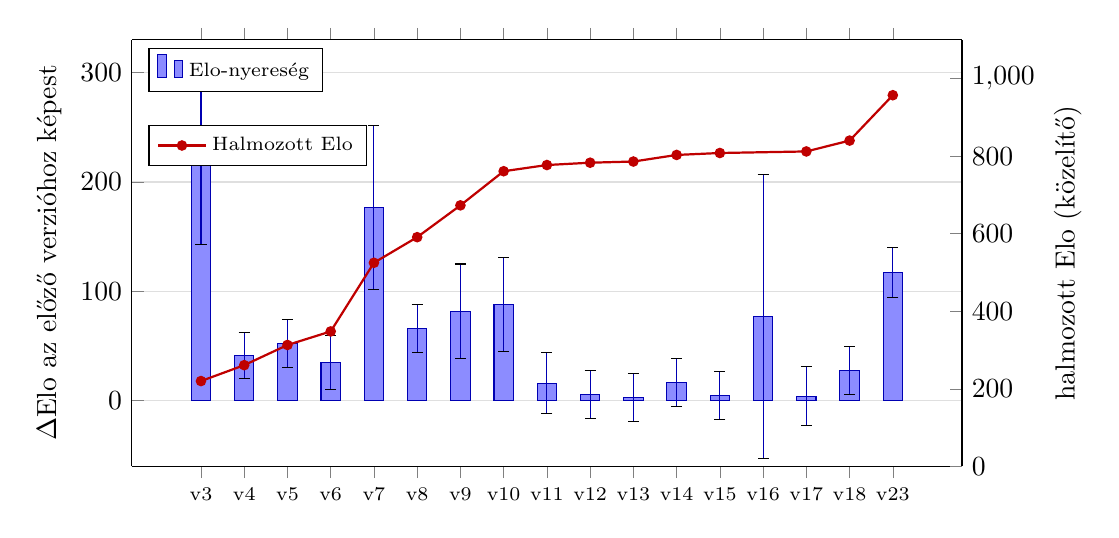
\begin{tikzpicture}
		\begin{axis}[
			width=\linewidth, height=7cm,
			ybar, bar width=7pt,
			ylabel={$\Delta$Elo az előző verzióhoz képest},
			symbolic x coords={v3,v4,v5,v6,v7,v8,v9,v10,v11,v12,v13,v14,v15,v16,v17,v18,v23},
			xtick=data, x tick label style={font=\scriptsize},
			ymin=-60, ymax=330,
			ymajorgrids, grid style={gray!25},
			axis y line*=left,
			legend style={at={(0.02,0.98)}, anchor=north west, font=\scriptsize},
		]
			\addplot[fill=blue!45, draw=blue!70!black, error bars/.cd, y dir=both, y explicit]
				coordinates {
					(v3,220) +- (0,77) (v4,41) +- (0,21) (v5,52) +- (0,22) (v6,35) +- (0,25)
					(v7,177) +- (0,75) (v8,66) +- (0,22) (v9,82) +- (0,43) (v10,88) +- (0,43)
					(v11,16) +- (0,28) (v12,6) +- (0,22) (v13,3) +- (0,22) (v14,17) +- (0,22)
					(v15,5) +- (0,22) (v16,77) +- (0,130) (v17,4) +- (0,27) (v18,28) +- (0,22) (v23,117) +- (0,23)
				};
			\addlegendentry{Elo-nyereség}
		\end{axis}
		\begin{axis}[
			width=\linewidth, height=7cm,
			symbolic x coords={v3,v4,v5,v6,v7,v8,v9,v10,v11,v12,v13,v14,v15,v16,v17,v18,v23},
			xtick=\empty, axis x line=none,
			axis y line*=right, ymin=0, ymax=1100,
			ylabel={halmozott Elo (közelítő)},
			legend style={at={(0.02,0.80)}, anchor=north west, font=\scriptsize},
		]
			\addplot[red!75!black, thick, mark=*, mark size=1.5pt]
				coordinates {
					(v3,220) (v4,261) (v5,313) (v6,348) (v7,525) (v8,591) (v9,673) (v10,761)
					(v11,777) (v12,783) (v13,786) (v14,803) (v15,808) (v17,812) (v18,840) (v23,957)
				};
			\addlegendentry{Halmozott Elo}
		\end{axis}
	\end{tikzpicture}
	\caption{Az egyes verziók erősödése az előző verzióhoz képest (oszlopok) és az ebből halmozott, közelítő Elo-nyereség (vonal). A v16 mérés csak 32 játszmából áll, ezért a halmozott értékbe nem számít bele.}
	\label{fig:versions}
\end{figure}

\Aref{fig:versions}.~ábra jól mutatja a fejlesztés két szakaszát. Az első napokban az alapvető technikák (TT, PVS és LMR, null-lépés, futility-vágások) egyenként is 35--220 Elo-pontot hoztak. A v11--v17 közötti módosítások már csak néhány Elo-pontos, a mérési hibán belüli javulást adtak; ezek nagy része tisztán sebesség- vagy robusztussági javítás volt (pl. TT-klaszterek, SEE-hibák javítása), amelyek a játékerőn rövid időkontrollal alig látszanak. A legnagyobb késői ugrást a v23 hozta: a zármentes transzpozíciós tábla, a nyugalmi keresésben is használt TT és az IIR együtt $+117$ Elo-pontot ért a közvetlen előd ellen. A közelítő halmozott nyereség a v2-től a v23-ig mintegy 950 Elo-pont; ez csak tájékoztató érték, mert a láncban a mérések nem mindig közvetlenül egymást követő verziók között történtek.

A legkorábbi, még a felülettel együtt fejlesztett keresőt (a v21 és v22 archív verziót, 2026.~április~21.) a fenti sorozat nem tartalmazza: ezeket csak néhány tucat, illetve négy próbajátszmával mértem, és a v1-ben a keresőt tudatosan egy minimális magról, lépésenként újraépítettem, hogy minden technika hatása külön mérhető legyen.


\section{Abszolút erősség: mérés a Stockfish ellen}\label{sec:stockfish}

A verziók közötti mérések csak relatív erősséget adnak. Az abszolút erősség becsléséhez a motort ismert erősségű ellenfél ellen kell játszatni. Erre a Stockfish~17.1~\cite{Stockfish} beépített erősségkorlátozását használtam (\texttt{UCI\_LimitStrength}, \texttt{UCI\_Elo}), amely a dokumentáció szerint a CCRL 40/4 (blitz) ranglistához~\cite{CCRL} van kalibrálva, 1320 és 3190 Elo között. A játszmákat a \emph{cutechess-cli}~\cite{CuteChess} vezérelte, a motor a konzolos backend UCI-kiszolgálóján keresztül játszott. Mindkét motor egy szálon, 128~MB hash-táblával, 10~s + 0,1~s időkontrollal futott; a kezdőállások a saját megnyitáskönyv véletlen állásai voltak, mindegyikből két játszmával, színcserével. A 300 játszma alatt egyetlen időtúllépés, szabálytalan lépés vagy összeomlás sem történt.

\begin{table}[!ht]
	\footnotesize
	\centering
	\begin{tabular}{l r r r c}
		\toprule
		Ellenfél (Stockfish 17.1) & Gy / V / D & Pontszám & $\Delta$Elo & Becsült erősség \\
		\midrule
		\texttt{UCI\_Elo} = 2600 & 92 / 5 / 3 & 93,5\% & $+463 \pm 157$ & $\approx 3063$ \\
		\texttt{UCI\_Elo} = 2900 & 62 / 17 / 21 & 72,5\% & $+168 \pm 67$ & $\approx 3068$ \\
		\texttt{UCI\_Elo} = 3190 & 15 / 34 / 51 & 40,5\% & $-67 \pm 48$ & $\approx 3123$ \\
		\bottomrule
	\end{tabular}
	\caption{A motor (,,Mester'' szint, HalfKAv2) eredményei a korlátozott erősségű Stockfish ellen, szintenként 100 játszma (Gy/V/D: a saját motor győzelmei, vereségei és döntetlenjei).}
	\label{tab:stockfish}
\end{table}

\Aref{tab:stockfish}.~táblázat szerint a 2600-as szint ellen a motor szinte minden játszmát megnyert; ilyen szélsőséges pontszámból az Elo-különbség csak pontatlanul becsülhető. A két informatív mérés (2900 és 3190) inverz varianciával súlyozott átlaga alapján a motor ereje \textbf{kb. 3100~$\pm$~40 Elo a CCRL blitz skálán}, és a három mérés egymással összhangban van. Az eredmény értelmezésénél figyelembe kell venni, hogy a Stockfish korlátozását 120~s + 1~s időkontrollal kalibrálták, a mérés viszont gyorsabb időkontrollal készült, ahol a korlátozott Stockfish valamivel gyengébben játszhat a névleges értékénél; másrészt a saját motor egy szálon futott, így több szálon ennél erősebb. A CCRL-értékek nem vethetők össze közvetlenül a FIDE-értékszámokkal, de ezen a szinten a motor bármely emberi játékosnál lényegesen erősebb.

\section{Mérések a konzolos backendben}\label{sec:terminal}

A végleges kereső erejét a konzolos backend robot-robot szimulációjával mértem két időkontrollal: mindkét félnek 10~másodperc alapidő lépésenként 0,1~másodperc bónusszal, illetve 60~másodperc alapidő 0,6~másodperc bónusszal. A szimuláció a megnyitáskönyvből választott kezdőállásokból színcserés párokban játszik, és a végén összesíti a győzelmeket, a döntetleneket és a pontszázalékot. \Aref{fig:terminal}.~ábra egy futás közbeni példakimenetet mutat.

\begin{figure}[!ht]
	\centering
	\screenshot{terminal_bot_measurement.png}{Konzolos robot-robot szimuláció kimenete futás közben.}{width=150mm,keepaspectratio}
	\caption{Példa a backend robot-robot szimulációjának futás közbeni kimenetére.}
	\label{fig:terminal}
\end{figure}

%----------------------------------------------------------------------------
\chapter{Összefoglalás és továbbfejlesztési lehetőségek}\label{chap:conclusion}
%----------------------------------------------------------------------------

\section{Az elvégzett munka értékelése}

A feladatkiírás minden pontját teljesítettem:
\begin{itemize}
	\item \emph{FIDE-szabályok és tündérsakk:} a motor a klasszikus szabályokat teljes egészében megvalósítja (sáncolás, en passant, átváltozás, ismétlés, ötvenlépéses szabály, elégtelen anyag), a tündérsakk alapelveit és az Amazon bábut \aref{chap:rules}.~fejezet mutatja be.
	\item \emph{Architektúra és UCI:} a rétegzett felépítésnek köszönhetően ugyanaz a motor fut konzolos UCI-kiszolgálóként és grafikus felülettel; a keresők egy közös interfész mögött cserélhetők és egymás ellen futtathatók.
	\item \emph{Klasszikus és új bábuk:} az Amazon sakk változat a lépésgenerálástól az értékelésig minden réteget érint, mégis néhány jól körülhatárolt módosítással illeszkedett, és a klasszikus játék működését bizonyíthatóan nem változtatta meg.
	\item \emph{Grafikus felület:} a Qt-alapú felület négy nehézségi szintet, sakkórát, visszavonást, visszajátszást és változatválasztást kínál.
	\item \emph{Mérések:} a lépésgenerálás helyességét perft-tesztek, a döntéshozatal hatékonyságát taktikai feladatok, több mint tizenkétezer verziók közötti mérőjátszma, valamint a korlátozott Stockfish elleni mérés igazolja, amely szerint a motor ereje kb. 3100 Elo a CCRL blitz skálán.
\end{itemize}

A legfontosabb tanulság a mérésvezérelt fejlesztés értéke volt. Több, papíron ígéretes ötlet (pl. a sakk-kiterjesztés) a mérésekben nem hozott javulást, míg más, látszólag apró változtatások (zármentes transzpozíciós tábla) jelentős erősödést okoztak. Automatikus verziózás és sok száz játszmás mérések nélkül ezek a döntések csak találgatások lettek volna.

\section{Továbbfejlesztési lehetőségek}

\begin{itemize}
	\item \emph{Általános tündérbábu-leírás:} jelenleg az Amazon kódba épített bábutípus. A következő lépés egy Betza-jelölésen alapuló, konfigurálható bábuleírás lehetne, amelyből a lépésgenerátor és a támadásszámítás automatikusan felépül, így új bábuk újrafordítás nélkül is felvehetők.
	\item \emph{Saját NNUE tanítása:} az Amazon értékét a motor jelenleg egy rögzített, $+300$ centigyalogos korrekcióval becsüli. Önjátszmákon tanított, az Amazont külön bemenetként kezelő háló pontosabb értékelést adhatna.
	\item \emph{UCI-opciók:} a hash-méret, a szálszám és a változat UCI \texttt{setoption} paranccsal is állíthatóvá tehető, és támogatható a \texttt{go depth}, \texttt{go infinite} és \texttt{ponder} mód.
	\item \emph{Pontosabb erősségmérés:} a Stockfish elleni mérést érdemes lenne a kalibráció időkontrolljával (120~s + 1~s), több szálon és több játszmával megismételni, valamint az Amazon változatban is elvégezni (pl. a Fairy-Stockfish ellen).
\end{itemize}


% Bibliography
%~~~~~~~~~~~~~~~~~~~~~~~~~~~~~~~~~~~~~~~~~~~~~~~~~~~~~~~~~~~~~~~~~~~~~~~~~~~~~~~~~~~~~~
\addcontentsline{toc}{chapter}{\bibname}
\bibliography{bib/mybib}

% Appendix
%~~~~~~~~~~~~~~~~~~~~~~~~~~~~~~~~~~~~~~~~~~~~~~~~~~~~~~~~~~~~~~~~~~~~~~~~~~~~~~~~~~~~~~
%----------------------------------------------------------------------------
\appendix
%----------------------------------------------------------------------------
\chapter*{\fuggelek}\addcontentsline{toc}{chapter}{\fuggelek}
\setcounter{chapter}{\appendixnumber}
\numberwithin{equation}{section}
\numberwithin{figure}{section}
\numberwithin{lstlisting}{section}

\input{include/\AIdeclaration}


\end{document}
